  %  This Script provides the Treasurer Dept
  %  Forfeiture Data Collection Mobile App Subsection
  %  Or Can compile alone with the commented texts toggled
%+++++++++++++++++++++++++++++++++++++++++++++++++++++++++++++++++++
%    To Do:
%  20200410 Notes
% Around line 519 Editing Admin manual
%
%-------------------------------------------------------------------
% OPTIONAL PREAMBLE FOR LOCAL COMPILE  %
  %
\def\titlename{Forfeiture Mobile App}
\def\authorName{Allegan County GIS Services}
\def\pdfTitle{Forfeiture Mobile App}
\def\pdfSubject{GIS Tools} %
\def\pdfKeywords{mobile,gis}

%+++++++++++++++++++++++++++++++++++++++++++++++++++++++++++++++++++
%  Used in Subsections that are capable of being compiled alone
%
%
%-------------------------------------------------------------------
\documentclass[letterpaper, 12pt]{memoir}
 %
\usepackage{import} % Required for importing other .tex docs.  (import uses everything bw Begin and End Doc)
\usepackage{float} % Required for specifying the exact location of a figure or table
\usepackage{graphicx} % Required for including images
\usepackage{wrapfig}
\usepackage[pdftex,breaklinks,colorlinks=true,linkcolor=black,citecolor=blue,urlcolor=red,linktocpage=false,pagebackref=true,filecolor=magenta]{hyperref}%http://www.tug.org/applications/hyperref/manual.html#x1-100003.6
\usepackage{cite}
\usepackage[toc,title,page]{appendix}
\usepackage{pdfpages} % enables loading a pdf into the doc
\usepackage{makeidx}
\usepackage{glossaries} % must be after hyperref
\usepackage{blindtext}
\usepackage{enumitem}
%\usepackage{caption}

%\setlist[description]{leftmargin=\parindent,labelindent=\parindent}

%\renewcommand*{\bibname}{References} % renames the bibliography

\newcommand{\HRule}{\rule{\linewidth}{0.5mm}} % Command to make the lines in the title page

\graphicspath{{img/}{GIS_ChampionSection/img/}{awardsChapter/GIS_ChampionSection/img/}{brandPart/awardsChapter/GIS_ChampionSection/img/}{img/}{pairedProgSection/img/}{methodChapter/pairedProgSection/img/}{methodPart/methodChapter/pairedProgSection/img/}{documentationSection/img/}{methodChapter/documentationSection/img/}{methodPart/methodChapter/documentationSection/img/}{docStorageOrgSection/img/}{methodChapter/docStorageOrgSection/img/}{methodPart/methodChapter/docStorageOrgSection/img/}{QGisSection/img/}{toolsChapter/QGisSection/img/}{servicePart/toolsChapter/QGisSection/img/}{ESRISection/img/}{toolChapter/ESRISection/img/}{servicePart/toolChapter/ESRISection/img/}{../../../../source/}{../../source/}{servicePart/applicationsChapter/treasurerSection/img/}}

%\setlength\parindent{0pt} % eliminates indents

 %
%
%%%%%%%%%%%%%%%%%%%%%%%%%%%%%%%%%%%%%%%%%%%%%%%%%%%%%%%%%%%%%%
\graphicspath{{img/}{GIS_ChampionSection/img/}{awardsChapter/GIS_ChampionSection/img/}{brandPart/awardsChapter/GIS_ChampionSection/img/}{img/}{pairedProgSection/img/}{methodChapter/pairedProgSection/img/}{methodPart/methodChapter/pairedProgSection/img/}{documentationSection/img/}{methodChapter/documentationSection/img/}{methodPart/methodChapter/documentationSection/img/}{docStorageOrgSection/img/}{methodChapter/docStorageOrgSection/img/}{methodPart/methodChapter/docStorageOrgSection/img/}{QGisSection/img/}{toolsChapter/QGisSection/img/}{servicePart/toolsChapter/QGisSection/img/}{ESRISection/img/}{toolChapter/ESRISection/img/}{servicePart/toolChapter/ESRISection/img/}{../../../../source/}{../../source/}{servicePart/applicationsChapter/treasurerSection/img/}{servicePart/toolsChapter/gisAdminSection/img/}{gisAdminSection/img/}{servicePart/toolsChapter/bsaSupportSection/img/}{servicePart/toolsChapter/coreDataEditsSection/img/}{servicePart/toolsChapter/coreDataSchemaSection/img/}{../img}{servicePart/applicationsChapter/equalizationSection/img/}{servicePart/toolsChapter/pythonScriptsSection/img/}{servicePart/toolsChapter/ESRISection/img/}{servicePart/applicationsChapter/drainsSection/img/}}


%C:\AC\jalapeno\processing\servicePart\applicationsChapter\drainsSection\img

 %
%   This script does not require Memoir Class
%%%%%%%%%%%%%%%%%%%%%%%%%%%%%%%%%%%%%%%%%%%%%%%%%%%%%%%%%%%%
%+++++++++++++++++++++++++++++++++++++++++++++++++++++++++++++++++++
% Custom Color pallette
    % Blues
\definecolor{HeaderBlueA}{RGB}{85,125,161}
\definecolor{HeaderBlueB}{RGB}{53, 98, 138}
\definecolor{HeaderBlueC}{RGB}{31,78,121}  % HeaderBlue1
\definecolor{HeaderBlueD}{RGB}{16, 60, 99}
\definecolor{HeaderBlueE}{RGB}{4, 40, 72 }
    % Oranges
\definecolor{HeaderOrangeA}{RGB}{249, 161, 121}
\definecolor{HeaderOrangeB}{RGB}{214, 116, 72}
\definecolor{HeaderOrangeC}{RGB}{187, 84, 37}
\definecolor{HeaderOrangeD}{RGB}{152, 57, 14}
\definecolor{HeaderOrangeE}{RGB}{111, 35, 0}
    % Golds
\definecolor{HeaderGoldA}{RGB}{249, 218, 121}
\definecolor{HeaderGoldB}{RGB}{214, 180, 72}
\definecolor{HeaderGoldC}{RGB}{187, 151, 37}
\definecolor{HeaderGoldD}{RGB}{152, 119, 14}
\definecolor{HeaderGoldE}{RGB}{111, 84, 0}
    % Greens
    % option 1
% \definecolor{HeaderGreenA}{RGB}{14, 219, 76}
% \definecolor{HeaderGreenB}{RGB}{23, 179, 70}
% \definecolor{HeaderGreenC}{RGB}{31, 131, 61}
% \definecolor{HeaderGreenD}{RGB}{30, 92, 49}
% \definecolor{HeaderGreenE}{RGB}{21, 50, 30}
    % option 2 (triad of HeaderBlueC)
\definecolor{HeaderGreenA}{RGB}{82, 169, 136}
\definecolor{HeaderGreenB}{RGB}{49, 145, 109}
\definecolor{HeaderGreenC}{RGB}{25, 126, 88}
\definecolor{HeaderGreenD}{RGB}{10, 103, 68}
\definecolor{HeaderGreenE}{RGB}{0, 75, 47}
% Color triad based on HeaderBlue1
% http://paletton.com/

\definecolor{HyperlinkBlue1}{RGB}{64,172,209}
\definecolor{graphicOrange}{RGB}{255,153,51}
\definecolor{gisRed}{RGB}{244,66,66}
%-------------------------------------------------------------------

 %
%%%%%%%%%%%%%%%%%%%%%%%%%%%%%%%%%%%%%%%%%%%%%%%%%%%%%%%%%%%%%%%%%%%%%%%%%%%%
    % Sets sectioning Layout Properties
    %
    %
    %\setsecnumdepth{subsection} % turns on subsec numbering
    %
\setsecheadstyle{\scshape\color{HeaderOrangeA}} % default is \Large\bfseries
    %\setsecheadstyle{\scshape\color{HeaderOrangeB}}
    %
    % Subsection
\setsubsecheadstyle{\large\scshape\color{HeaderOrangeB}} % default is \large\bfseries
    %\setsubsecheadstyle{\huge\centering\color{HeaderOrangeE}}%
    % Subsubsection
\setsubsubsecheadstyle{\Huge\scshape\centering\color{HeaderBlueE}} % default is \bfseries
    %\setsubsubsecheadstyle{\LARGE\scshape\centering\color{HeaderBlueC}}%   1
    % Paragraph
\setparaheadstyle{\bfseries\Large\color{HeaderBlueC}}%
     %\setparaheadstyle{\Large\color{HeaderBlueA}}%2
     % Subparagraph
     %\setsubparaheadstyle{\large\color{HeaderBlueB}}%
\setsubparaheadstyle{\bfseries\large\color{HeaderOrangeB}}%
     %
     % \setbeforeSskip{<skip>} pg .95
     % The absolute value of the <skip> length argument is the space to leave above the heading.
     % If the actual value is negative then the first line after the heading will not be indented.
\setbeforesecskip{-35pt plus -10pt minus -2pt}
\setbeforesubsecskip{-32.5pt plus -10pt minus -2pt}
\setbeforesubsubsecskip{-32.5pt plus -10pt minus -2pt}
\setbeforeparaskip{-32.5pt plus -10pt minus -2pt}
\setbeforesubparaskip{-5pt plus -3pt minus -1pt}
    %
    % \setSindent{<length>}
    % The value of the length argument is the indentation of the heading (number and
    % title) from the lefthand margin. This is normally 0pt.
\setsubparaindent{0pt}
    % \setafterSskip{<skip>} pg.96
    % If the value of the <skip> length argument is positive it is the space to leave between the
    % display heading and the following text. If it is negative, then the heading will be runin
    % and the value is the horizontal space between the end of the heading and the following text.
    %
\setaftersecskip{.05in}
\setaftersubsecskip{.15in}
\setaftersubsubsecskip{.1in}
\setafterparaskip{.05in}
\setaftersubparaskip{.05in}
    %
\renewcommand{\partnamefont}{\color{HeaderOrangeE}\Huge\normalfont}
\renewcommand{\partnumfont}{\color{HeaderOrangeE}\Huge\normalfont}
    %
    % End of Setting sectioning Layout Properties
%%%%%%%%%%%%%%%%%%%%%%%%%%%%%%%%%%%%%%%%%%%%%%%%%%%%%%%%%%%%%%%%%%%%%%%%%%%%
\setlength\columnsep{.3in}

 %
%%%%%%%%%%%%%%%%%%%%%%%%%%%%%%%%%%%%%%%%%%%%%%%%%%%%%%%%%%%%
% HEADERS AND FOOTERS
%%%%%%%%%%%%%%%%%%%%%%%%%%%%%%%%%%%%%%%%%%%%%%%%%%%%%%%%%%%%
          %This script requires Memoir Class
    %  Page Styles
    %  In LATEX the page style refers to the part of the page building mechanism that
    %   attaches the headers and footers to the actual page.
%%%%%%%%%%%%%%%%%%%%%%%%%%%%%%%%%%%%%%%%%%%%%%%%%%%%%%%%%%%%
%  This block defines jalapenoPageStyleA page style
\makepagestyle{jalapenoPageStyleA}
    % headers
\makeheadrule {jalapenoPageStyleA}{\textwidth}{\normalrulethickness}
\makeheadfootruleprefix{jalapenoPageStyleA}{\color{HeaderOrangeE}}{\color{HeaderOrangeE}}
\makeevenhead {jalapenoPageStyleA}{\helv \thepage}{} {\helv \rightmark}
\makeoddhead {jalapenoPageStyleA}{\helv \leftmark}{}{\helv \thepage}
    % footers
\makefootrule {jalapenoPageStyleA}{\textwidth}{\normalrulethickness}{\footruleskip}
\makeevenfoot {jalapenoPageStyleA}{}{} {}
\makeoddfoot {jalapenoPageStyleA}{}{} {}
    %
%%%%%%%%%%
    %
%  This block defines marks for jalapenoPageStyleA page style
    %  See page 11 of Page Styles in Memoir
    %
\makeatletter % because of \@chapapp
%
\makepsmarks {jalapenoPageStyleA}{
%\nouppercaseheads
\createmark {chapter} {both} {shownumber}{\@chapapp\ }{. \ } % set leftmark to chapter
%\createmark {section} {right}{shownumber}{} {. \ }
\createmark {subsection} {right}{shownumber}{} {. \ } % set rightmark to subsection
%\createmark {subsubsection}{right}{shownumber}{} {. \ } % set rightmark to subsubsection
\createplainmark {toc} {both} {\contentsname}
\createplainmark {lof} {both} {\listfigurename}
\createplainmark {lot} {both} {\listtablename}
\createplainmark {bib} {both} {\bibname}
\createplainmark {index} {both} {\indexname}
\createplainmark {glossary} {both} {\glossaryname}

}
\makeatother
%  End of jalapenoPageStyleA pagestyle
%%%%%%%%%%%%%%%%%%%%%%%%%%%%%%%%%%%%%%%%%%%%%%%%%%%%%%%%%%%%

%%%%%%%%%%%%%%%%%%%%%%%%%%%%%%%%%%%%%%%%%%%%%%%%%%%%%%%%%%%%
%  This block defines emptyPageStyle page style
\makepagestyle{emptyPageStyle}
    % headers
\makeevenhead {emptyPageStyle}{}{}{}
\makeoddhead {emptyPageStyle}{}{}{}
    % footers
\makefootrule {emptyPageStyle}{}{}{}
\makeevenfoot {emptyPageStyle}{}{}{}
\makeoddfoot {emptyPageStyle}{}{}{}
    %
%%%%%%%%%%
\newcommand{\normPageLayout}{%
\setmarginnotes{.2in}{.5in}{.1in}%
\setlrmarginsandblock{*}{0.3\paperwidth}{.75}% Left right ratio
\setulmarginsandblock{1in}{*}{*}%
\checkandfixthelayout%
\clearpage}

\newcommand{\widePageLayout}{%
\setmarginnotes{.1mm}{.1mm}{.1mm}%
\setlrmarginsandblock{1in}{1in}{*}% Left right ratio
\setulmarginsandblock{1in}{1in}{*}%
\checkandfixthelayout%
\clearpage}

 %
%%%%%%%%%%%%%%%%%%%%%%%%%%%%%%%%%%%%%%%%%%%%%%%%%%%%%%%%%%%%%%%%%%%%%%%%%%%%
  % beginning od customchpstyle
    %
\makeatletter % handler for @
    %
\makechapterstyle{jalapenoChapterStyle}{%
    %
    \newlength{\chapColorbarheight}
    \setlength{\chapColorbarheight}{.06in}		% Setting the height of the bar
    %
    \newlength{\chapnumboxlength}
    \setlength{\chapnumboxlength}{.75in}	% Setting the length of the box containing chapter number
    %
    \newlength{\leftbarlength}
    \setlength{\leftbarlength}{.5in}  		% Setting length of the bar left to the chapter number
    \setlength{\afterchapskip}{.5in}
    \renewcommand*{\chapterheadstart}{\vspace*{.25in}} % vspace from top of page
    \renewcommand*{\afterchapternum}{\vspace*{-.9in}} % neg moves chapter title above chapter number
    \renewcommand*{\chapnumfont}{\slshape} % Number Font
    \renewcommand*{\chaptitlefont}{\flushright\color{HeaderOrangeE}\slshape\huge}
    \renewcommand*{\printchaptername}{} % sets the text in brackets before the number
    %\makeatletter
    \newcommand*{\thickrulefill}{\leavevmode \leaders \hrule height \chapColorbarheight \hfill \kern \z@} % rightbar length setter
    %\makeatother
    \renewcommand*{\printchapternum}{%
        %\makebox[0pt][l]{%
        \color{HeaderOrangeE}
        \rule{\leftbarlength}{\chapColorbarheight} % Left bar
        \quad % hspace
        \resizebox{!}{\chapnumboxlength}
        {\chapnumfont \thechapter} % Chapter name and number
        \quad % hspace
        \color{HeaderOrangeE}\thickrulefill % implements thickrulefill
     } %
     \makeatother % closes handler for @
} % End of customchpstyle
%%%%%%%%%%%%%%%%%%%%%%%%%%%%%%%%%%%%%%%%%%%%%%%%%%%%%%%%%%%%%%%%%%%%%%%%%%%%

 %
%\newglossaryentry{ex}{name={sample},description={an example}}


\newglossaryentry{projection}{name={map projection},description={Representing a sphere on a flat surface}}
 %
\newlength\drop
\makeatletter
\newcommand*\titleM{\begingroup% Misericords, T&H p 153
\setlength\drop{0.08\textheight}
\centering
\vspace*{\drop}
{\protect\HRule}
\begin{figure}[H] % included image
\begin{center}	% centered horizontally
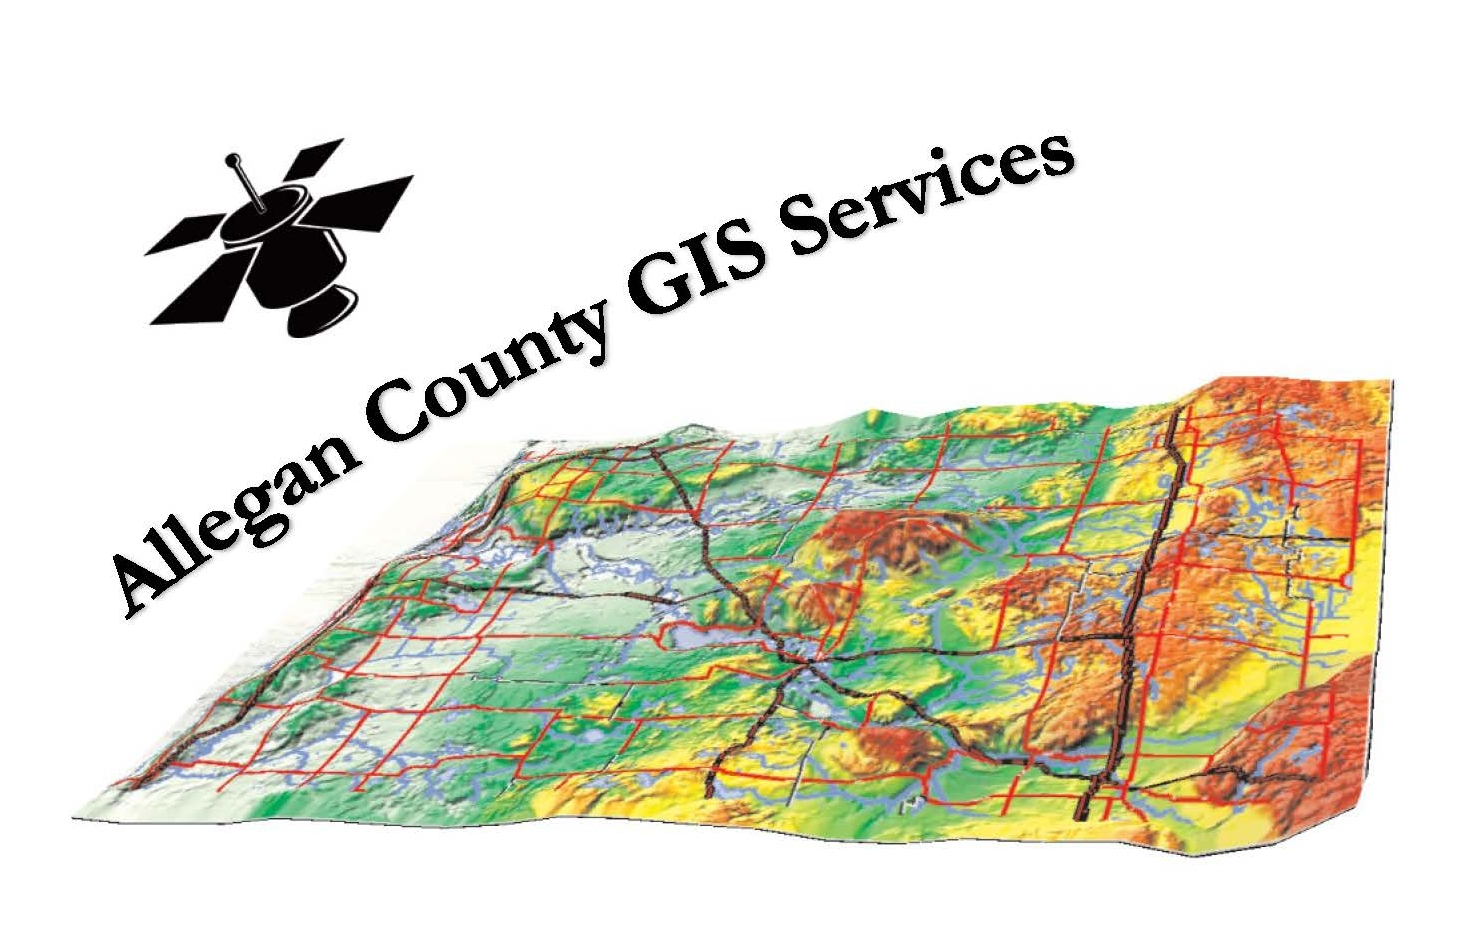
\includegraphics[scale=.5]{GIS_Logo_better.jpg}
\end{center}
\end{figure}
\vspace{-.1in}
{\Huge\bfseries\titlename}\\[2\baselineskip]
{\protect\HRule}\\[\baselineskip]
{\small\scshape www.allegancounty.org/gis}\\[2\baselineskip]
{\small\scshape \@date}\par
\endgroup}
\makeatother
  % inputs common title
  % SET PDF METADATA  %
\hypersetup{pdfauthor={\authorName},
pdftitle={\pdfTitle}, %  Sets PDF properties
pdfsubject={\pdfSubject},
pdfkeywords={\pdfKeywords}}
%-------------------------------------------------------------------
  % TOC DEPTH  %
\setcounter{tocdepth}{5}  % Sets Table of Contents level to show
                             % subparagraphs(5), paragraphs(4),
                             % subsubsections(3), subsections(2(default)),
                             % sections(1), chapters and parts(0)
 %
%+++++++++++++++++++++++++++++++++++++++++++++++++++++++++++++++++++
%    SET TEXT BLOCK AND MARGINS FOR COVER PAGE  %
\setmarginnotes{.1in}{.4in}{.1in}
\setlrmarginsandblock{*}{0.18\paperwidth}{1} % Left right ratio
\setulmarginsandblock{1in}{1in}{*}
\checkandfixthelayout
\makeatletter
\ch@ngetext
\makeatother
  %+++++++++++++++++++++++++++++++++++++++++++++++++++++++++++++++++++
	%  Front Section
  %-------------------------------------------------------------------
\begin{document}% document begins
   %
\frontmatter % turns off chapter numbering and uses roman numerals for page numbers
   %
\pagestyle{plain}
   %
\begin{titlingpage}
   %
\titleM  % Inputs titleM
   %
\end{titlingpage}
   %
%+++++++++++++++++++++++++++++++++++++++++++++++++++++++++++++++++++
%    SET TEXT BLOCK AND MARGINS FOR MAIN DOCUMENT PAGES   %
\setmarginnotes{.1in}{.4in}{.1in}
\setlrmarginsandblock{*}{0.18\paperwidth}{.75} % Left right ratio
\setulmarginsandblock{1in}{1in}{*}
\checkandfixthelayout
\makeatletter
\ch@ngetext
\makeatother
%-------------------------------------------------------------------
\tableofcontents % creates TOC
  %
%+++++++++++++++++++++++++++++++++++++++++++++++++++++++++++++++++++
%		Main Section
%-------------------------------------------------------------------
\mainmatter % turns on chapter numbering, resets page numbering and uses arabic numerals for page numbers
  %
\chapterstyle{jalapenoChapterStyle} % custom from chapterStyles.tex
  %
\pagestyle{jalapenoPageStyleA} % custom from pageStyles.tex

  %
%-------------------------------------------------------------------
    %
    %
%\begin{document}% document begins
 %
 %--------------------------------------------------
\subsection{Forfeiture Data Collection}
  %
\subsubsection{Problem and Analysis}
  %
\begin{adjmulticols}{2}{\innerMar}{\outerMar}
  %
\paragraph{Background}
  %
\noindent Treasurer department has an annual responsibility to properly document the tax forfeiture process.  The LIS Department built an application in MS Access and MapInfo that consumed a daily export from BSA and was deployed to the field on a laptop.  A digital camera was used for site photos and later imported into the laptop.
  %
\paragraph{Statement of Problem}
  %
\noindent The current Tax Forfeiture workflow is built on MapInfo software and MS Access amd executed on a laptop pc.  Both MapInfo and MS Access are no longer supported in county workflows.  ESRI software can be used to rebuild the workflow.  \textit{Forfeiture Data Collector Application}, (\textbf{Forfeiture App}) must be recreated in the ESRI framework.
  %
\paragraph{Analysis}
  %
\noindent \textbf{Forfeiture App} will facilitate: \textit{Mobile data collection on a handheld device},: (\textbf{Mobile Interface}) and an
  %
\textit{in office workflow to complete data processing}, (\textbf{Pre and PostProcessing})
  %
\subparagraph*{Mobile Interface}
  %
\begin{itemize} %
  %
\item Synchronize with data in the office (online)
  %
\item Collect data and photos of forfeiture sites (offline)
  %
\item Synchronize the collected data with data in the office (online)
  %
\end{itemize} %
  %
\subparagraph*{Pre \& Post Processing}
  %
\begin{itemize} %
  %
\item Produce and print a form for each site visited with required data and images
  %
\end{itemize} %
  %
\end{adjmulticols}
  %
\clearpage
   %
   %
 \subsubsection{Design Overview}
   %
   % Single Figure
   %
 \marginpar{\marginText Forfeiture Parcels is used through the workflow}
 %\marginpar{\color{graphicOrange}\textbf{Forfeiture Parcels} is used through the workflow}
 \vspace{-.2in}

 \begin{figure}[h!]
 \centering
     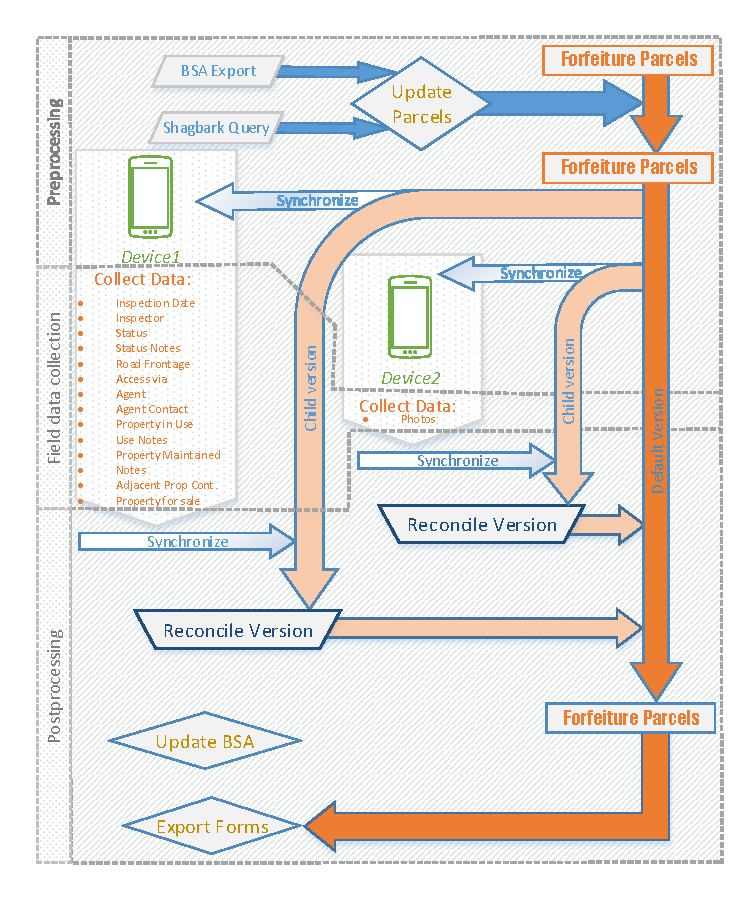
\includegraphics[width=1\textwidth]{ProjectDesign}
 \vspace{-.2in}

 \caption{Project Design}
 \end{figure}
   %
 \clearpage
   %
   %
 \paragraph{Forfeiture App Summary}
 \vspace{.25in}

 There are {\LARGE three parts} to the daily routine:
 \vspace{.25in}

 \begin{enumerate}
 \item \Large Preprocessing \normalsize(in the office):
   %
 \begin{itemize}
 \item Export current forfeiture list from BSA
 \item Update Forfeiture Parcels with BSA export
 \item Update Forfeiture Parcels with contaminated sites information
 \item Synchronize Forfeiture Parcels to Mobile Interface
 \end{itemize}
   %
 \item \Large Field data collection \normalsize with Mobile Interface:
   %
 \begin{itemize}
 \item Aids in navigation
 \item Provides a Checklist of data points for each site
 \item Attaches photos for each site
 \item Save results for synchronization in post-processing
 \end{itemize}
   %
 \item \Large Post-processing \normalsize (in the office)
   %
 \begin{itemize}
 \item Synchronize data and images collected in Mobile Interface to Forfeiture Parcels
 \item Export form for each site
 \item Print form for each site
 \item Update BSA data
   %
 \end{itemize}
   %
 \end{enumerate}
   %
 \clearpage
    %
    %
  \paragraph{Technologies Used in The Forfeiture App}
    %
  \begin{adjmulticols}{2}{\innerMar}{\outerMar}
    %
  \subparagraph{BSA Data}
    %
  \noindent Details of parcels in the forfeiture process are managed in BSA Delinquent Tax.net.  The Treasurer office does a BSA export of the parcels in need of a site visit in the preprocessing.
    %
  \subparagraph{ArcGIS Desktop}\noindent Tools are designed to preprocess and postprocess forfeiture parcel data for fieldwork.  The user will execute a preprocess script tool that prepares the data for field deployment.  After fieldwork, a post process script tool synchronizes data from the fieldwork with the live data on the Allegan County network.
    %
  \subparagraph{ArcGIS Collector}\noindent A free mobile application developed and tested on Android is deployed to the field for data collection.  The application is configured to work offline(without an internet or cellular connection) by syncronizing before and after fieldwork. The user collects the necessary information on each forfeiture parcel in the field disconnected, and then uploads the changes when reconnected.
    %
  \subparagraph{Enterprise Geodatabse}\noindent Live data from a publishing geodatabase (ACPub), running on SQL Server database server (acintsql01) provides access to Forfeiture Parcels
    %
  \subparagraph{ArcGIS Portal} \noindent Forfeiture Parcels is served as a feature service (REST service)  named TaxReversionParcels.  A webmap on Portal, called the Forfeiture Field Map consumes the TaxReversionParcels exposing the data to editing.  The Forfeiture Field Map is configured to work in the ArcGIS Collector App.
    %
  \end{adjmulticols}
    %
    % Single Figure
    %
  \begin{figure}[H]
  \centering
      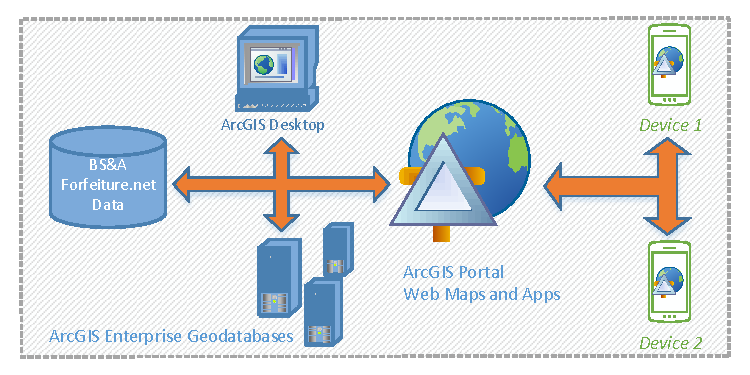
\includegraphics[width=.9\textwidth]{TechFlowChart}
  \vspace{-.25in}

  \caption{Technology Design}
  \end{figure}
  \clearpage
    %
    %
  \subsubsection[Data Details]{Data Details\texorpdfstring{\\}{}}
    %
  \noindent The data is located in a geodatabase called ACPUB.  ACPUB is on SQL Server ACINTSQL01.
    %
    % Two Figures Wrapped
    %
  \begin{wrapfigure}{r}{0.6\textwidth}
  \centering
      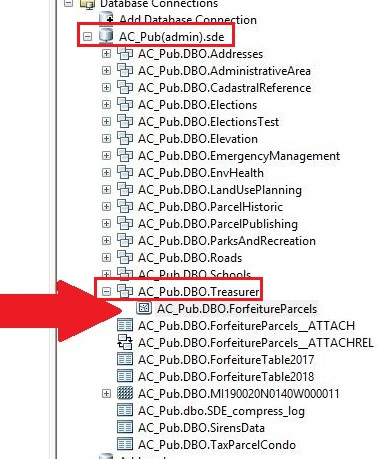
\includegraphics[width=.5\textwidth]{LiveDataLocation}
  \caption{Live Data Location}
  \vspace{1in}

  \HRule
  %\\[.2cm] % Horizontal Line added
  \vspace{1in}

      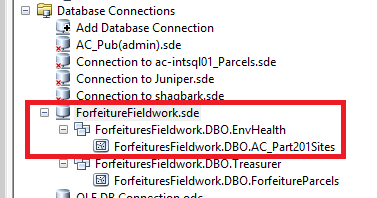
\includegraphics[width=.5\textwidth]{contaminationFeatureClass.png}
 \vspace{-.1in}
 \caption{Contamination Feature Class}
  \end{wrapfigure}
    %
  \vspace{1in}

  Forfeiture Parcels Data
  \vspace{4in}

  Contamination Data
  \clearpage
    %
    %
  \paragraph{ForfeitureParcels Feature Class Details}
  \vspace{.5in}

  \begin{table}[htbp]
  \centering
  \resizebox{\linewidth}{!}{%
  \begin{tabular}{|l|l|c|r|}
  \hline
  \multicolumn{4}{|c|}{{\LARGE Attribute Details}} \\
  \hline
  Field Name&Field Alias&Entry Type&Note\\ \hline
  PropertyNumber&Property Number&Prefilled&NA\\
  Need2Print&Print Today&Dropdown&{\tiny Yes or No}\\
  InspectionDate&Inspection Date&{\tiny Autofill or Dropdown}&NA\\
  Inspector&Inspector&Dropdown&NA\\
  Address&Address&Prefilled&NA\\
  Status&Status&Dropdown&NA\\
  StatusNotes&Status Notes&Open Entry&120Char\\
  Roadfrontage&Road Frontage&Dropdown&{\tiny Yes or No}\\
  AccessVia&Access Via&Open Entry&30Char\\
  Agent&Agent&Open Entry&30Char\\
  AgentContact&Agent Contact&Open Entry&30Char\\
  PictureComments&Picture Comments&Open Entry&50Char\\
  PropertyInUse&Property In Use&Dropdown&{\tiny Yes or No}\\
  UseNotes&Use Notes&Open Entry&120Char\\
  {\tiny PropertyMaintained}&{\tiny Property Maintained}&Dropdown&{\tiny Yes or No}\\
  PropMaintNotes&{\tiny Property Maintained Notes}&Open Entry&120Char\\
  {\tiny PropertyContaminated}&{\tiny Property Contaminated}&Prefilled&{\tiny Preprocessing}\\
  {\tiny PropertyContaminatedNotes}&{\tiny PropertyContaminatedNotes}&Prefilled&{\tiny Preprocessing}\\
  {\tiny AdjacentPropertyContaminated}&{\tiny Adjacent Property Contaminated}&Prefilled&{\tiny Preprocessing}\\
  {\tiny AdjPropertyContaminatedNotes}&{\tiny Adj Property Contaminated Notes}&Prefilled&{\tiny Preprocessing}\\
  PropertyForSale&Property For Sale&Dropdown&{\tiny Yes or No}\\
  GlobalID&GlobalID&NA&NA\\
  PostedDate&Posted Date&Dropdown&Date\\
  Posted&Posted&Prefilled&NA\\
  InList&In List&Prefilled&{\tiny Preprocessing}\\
  PostedInList&Posted In List&Prefilled&{\tiny Preprocessing}\\
  Acres&Acres&Prefilled&NA\\
  Class&Class&Prefilled&NA\\
  \hline
  \end{tabular}
  }
  \caption{Dataset Details}
  \end{table}
  \clearpage
    %
    %
  \paragraph{Webmap Details}The Forfeiture Field Map is made up of a feature layer and a basemap.
    %
    % Double Figure No Wrap
    %
  \begin{figure}[h!]
  \centering
      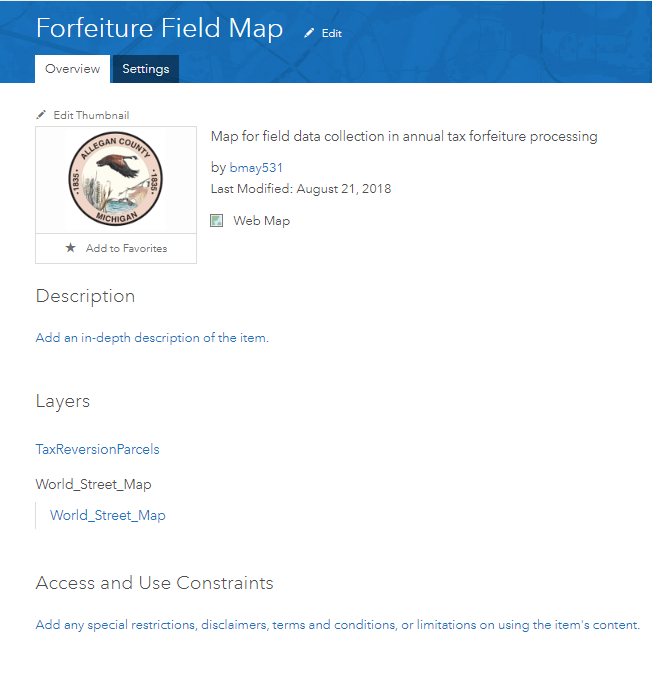
\includegraphics[width=.55\textwidth]{webMapDetails}
  \vspace{-.25in}

  \caption{Web Map Details}
  \end{figure}
    %
  \subparagraph{Feature Layer Details}TaxReversionParcels has been configured for offline use.
  \begin{figure}[h!]
  \centering
      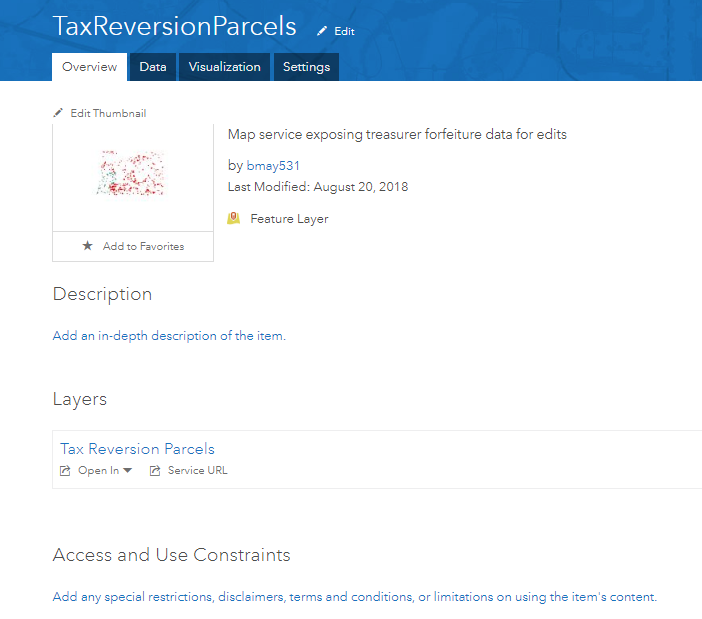
\includegraphics[width=.55\textwidth]{layerDetails}
  \vspace{-.15in}

  \caption{Feature Layer Details}
  \end{figure}
    %
  \clearpage
    %
    %
  %images of publishing the service and explanation of settings required for offline use
    %
  \subparagraph{Basemap Details}
  \begin{itemize}
    \setlength\itemsep{.3in}
    \item A tiled basemap service is used
    \item The infoserv user credentials are used for sharing
    \item The url for the shared service is:
  \end{itemize}
    %

 \noindent \textcolor{HyperlinkBlue1}{\scriptsize\path{https://tiledbasemaps.arcgis.com/arcgis/rest/services/World_Street_Map/MapServer}}
 \vspace{.5in}

    %
    % Single Figure
    %
  \begin{figure}[h!]
  \centering
  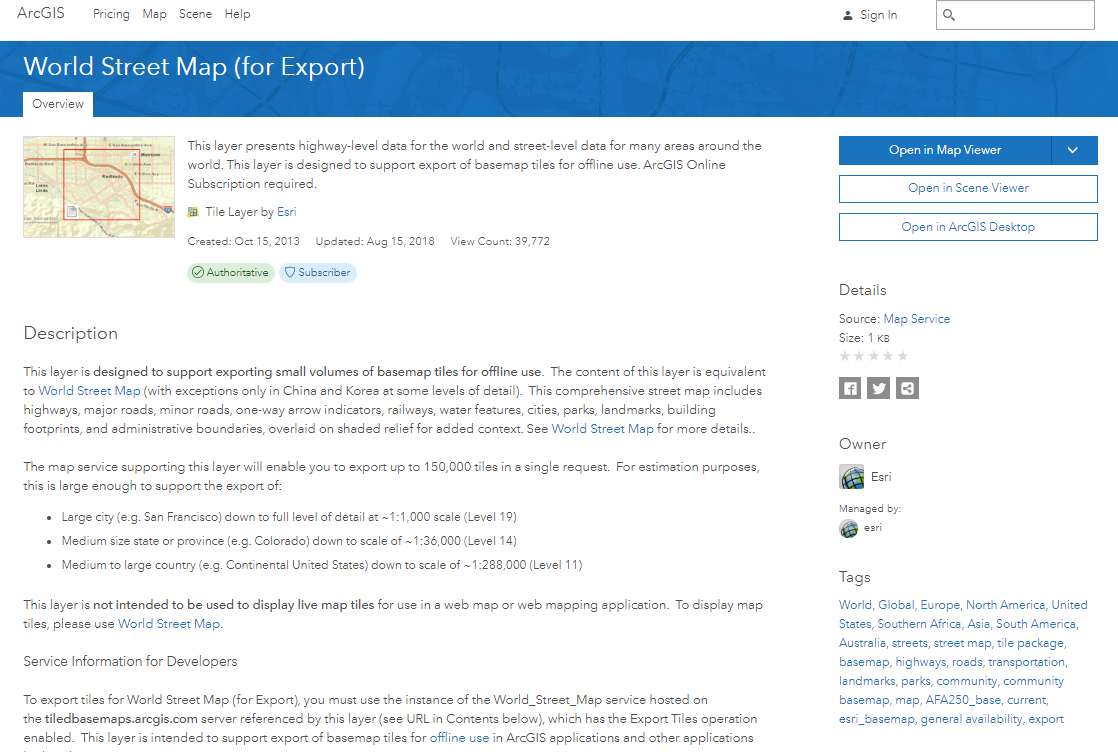
\includegraphics[width=1\textwidth]{BasemapSourceDescription}
  \caption{Basemap Source Description}
  \end{figure}
  \clearpage
    %
      %
  \subsubsection{Hard Copy Record}
  screenshots:
  arcmap map
  arcmap tools
  portal screenshots
  sql server mgt screen shots
  phone screenshots
    %
  \paragraph{ArcGIS Server}
  \clearpage
    %
    %
  \subsubsection{Administrative Manual}

  \paragraph{Annual Setup}

  A new dataset for forfeiture parcels must be created each year.

  \noindent The forfeiture information comes from BSA Forfeitures.net.

  \noindent Parcel geometry and other attributes comes from ACParcelsCombined.



 \subparagraph{To Connect to the Forfeiture Dataset}

  \noindent{To Add a new database connection:}
  \begin{itemize}
  \item {\Large Right Click on Add Database Connection}

  \begin{itemize}
  \item {\Large Enter these values into the tool}
  \end{itemize}
  \end{itemize}

  \vspace{.1in}

    %
    % Single Figure No Wrap
    %
  \begin{figure}[h!]
  \centering
      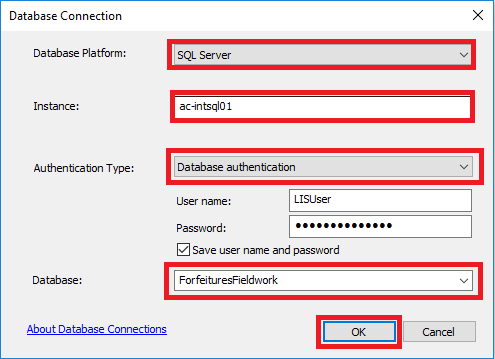
\includegraphics[width=.8\textwidth]{newConnection.PNG}
  \caption{Add New Connection}
  \end{figure}
  \vspace{.15in}

 {\bigbtn Push \fbox{OK}}

 \clearpage


  \subparagraph{Update the Forfeiture Dataset}

  \noindent{To clear the features from the existing dataset:}
  \begin{itemize}
  \item {\Large Use the Delete Feature Tools}
  \item {\Large For Input Features:}
  \begin{itemize}
  \item {\Large ForfeituresFieldwork.DBO.ForfeitureParcels}
  \end{itemize}
  \end{itemize}

  \vspace{.1in}

    %
    % Single Figure No Wrap
    %
  \begin{figure}[h!]
  \centering
      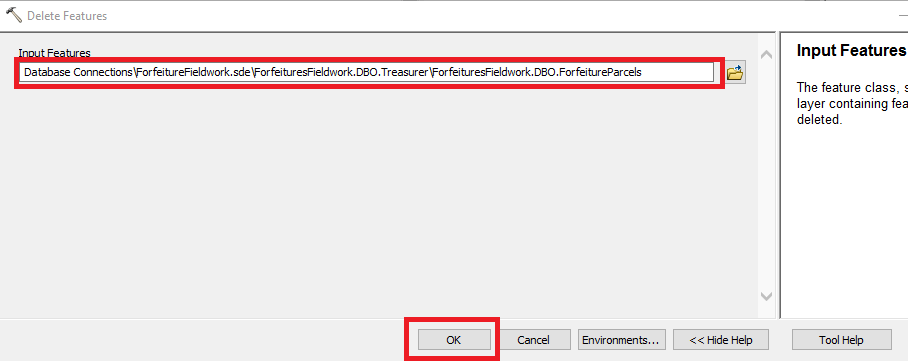
\includegraphics[width=.7\textwidth]{AnnualDeleteFeatures.png}
  \caption{Annual Delete Features}
  \end{figure}
  \vspace{.15in}

 {\bigbtn Push \fbox{OK}}


 \subparagraph{Delete the attached table}
  \begin{figure}[h!]
  \centering
      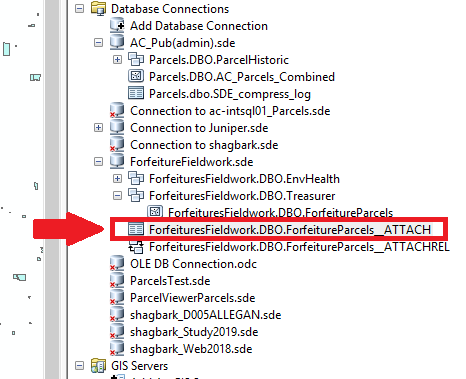
\includegraphics[width=.4\textwidth]{deleteAttachedTable.PNG}
  \caption{Delete Attached Table}
  \end{figure}

  \clearpage






















 \paragraph{Create new connection to BSA server}

  A connection to BSA is used to get the latest forfeiture information.

 \subparagraph{To Connect to the BSA Server}

  \noindent{To Add a new database connection:}
  \begin{itemize}
  \item {\Large Right Click on Add Database Connection}

  \begin{itemize}
  \item {\Large Enter these values into the tool}
  \end{itemize}
  \end{itemize}

  \vspace{.1in}

    %
    % Single Figure No Wrap
    %


 \begin{figure}[h!]
  \centering
      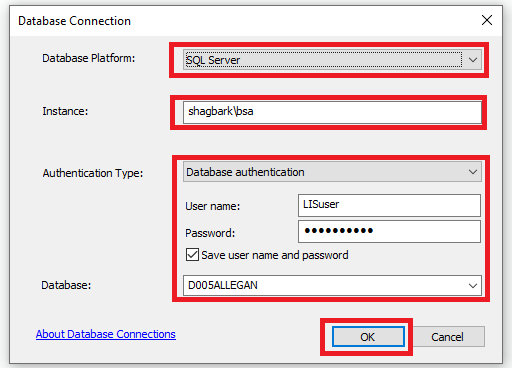
\includegraphics[width=.8\textwidth]{shagbarkBsaConnection.PNG}
  \caption{Connect to BSA Server}
  \end{figure}

  \vspace{.15in}

 {\bigbtn Push \fbox{OK}}

 \clearpage





      %
      %
  \paragraph{Create a Table Query For the New Data}
  %\vspace{.25in}

  \begin{itemize}
  \item {File {\menuArrow} Add Data {\menuArrow} Add Query Layer}
  \item {{ Select your connection} (\textit{shagbark\_D005ALLEGAN.sde})}
  \end{itemize}
    %
    % Single Figure No Wrap
    %
  \begin{figure}[h!]
  \centering
      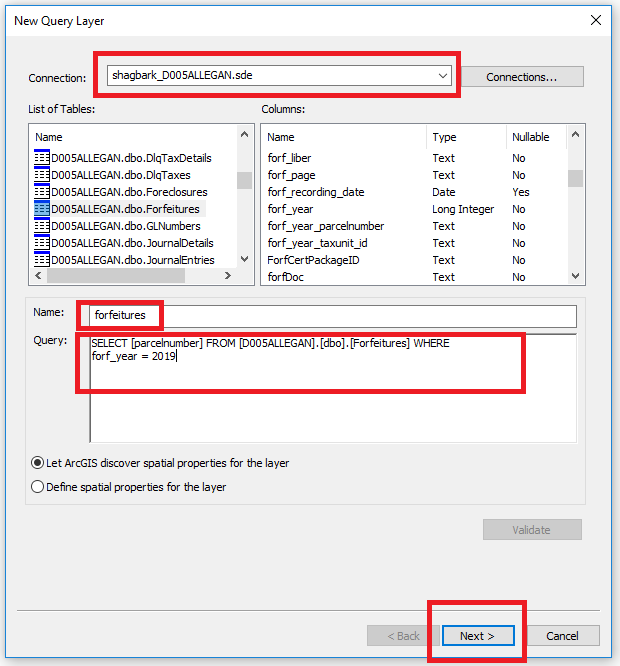
\includegraphics[width=.9\textwidth]{ForfeitureQueryLayerDetails.PNG}
  \caption{New Query Layer Dialog}
  \end{figure}
    %
 \vspace{.1in}
 Edit Query Text for current Year:
 \vspace{.1in}
  \begin{verbatim}
  SELECT [parcelnumber] FROM [D005ALLEGAN].[dbo].[Forfeitures]
  WHERE forf_year = 2020
  \end{verbatim}
    %
    %
  %\clearpage
    %
    %
  \subparagraph{Select a Unique Identifier}
    %
    %
    % Single Figure No Wrap
    %
  \begin{figure}[h!]
  \centering
      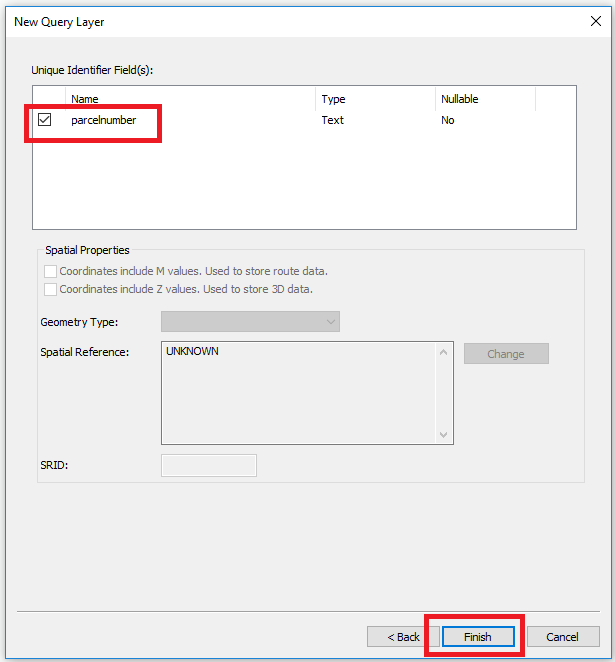
\includegraphics[width=.95\textwidth]{ForfeitureQueryLayerUID.PNG}
  \caption{Query Layer Unique ID}
  \end{figure}
    %
 {\bigbtn Push \fbox{Finish}}

  \clearpage
    %
    %
  \subparagraph*{Table is added to the map}
    %
    % Single Figure No Wrap
    %
  \begin{figure}[h!]
  \centering
      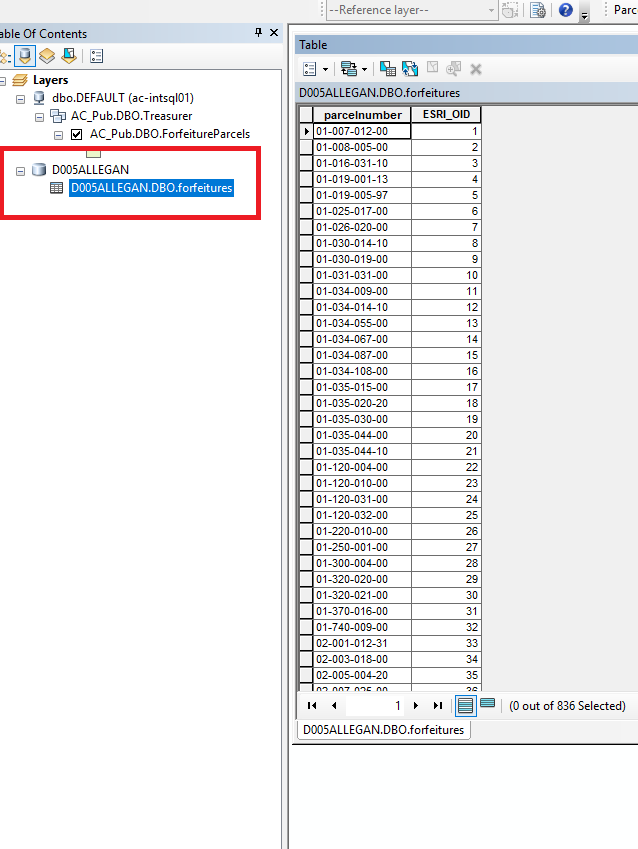
\includegraphics[width=.95\textwidth]{forfeituresTableAdded.PNG}
  \caption{Forfeiture Table Added}
  \end{figure}
  \clearpage
    %
    %
  \paragraph{Add Parcels Layer to the Map}
 %\vspace{.3in}

  \begin{itemize}
  \item {Parcels are added to the map to provide parcel geometry and attributes}
  \item {Parcel year is = current year - 2}
  \item {I.E. Use ACParcelsCombHistoric2018 in 2020}
  \end{itemize}

  \vspace{.25in}

    %
    % Single Figure No Wrap
    %
  \begin{figure}[h!]
  \centering
      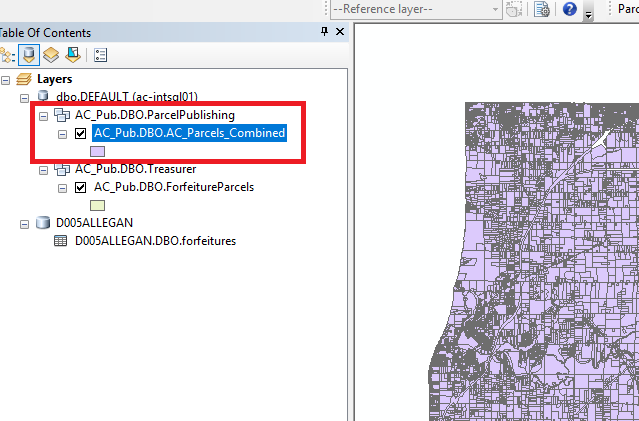
\includegraphics[width=.95\textwidth]{ParcelLayerAdded.PNG}
  \caption{Parcels Layer Added}
  \end{figure}
  \clearpage







   \paragraph{Forfeiture parcel missing spatial data}

   \subparagraph*{A temporary join, selection, and export will save these}

   \vspace{.3in}

  \begin{itemize}
  \item {Join Parcels to Forfeiture table}

  %\end{itemize}

  %\vspace{.25in}

    %
    % Single Figure No Wrap
    %
  \begin{figure}[h!]
  \centering
      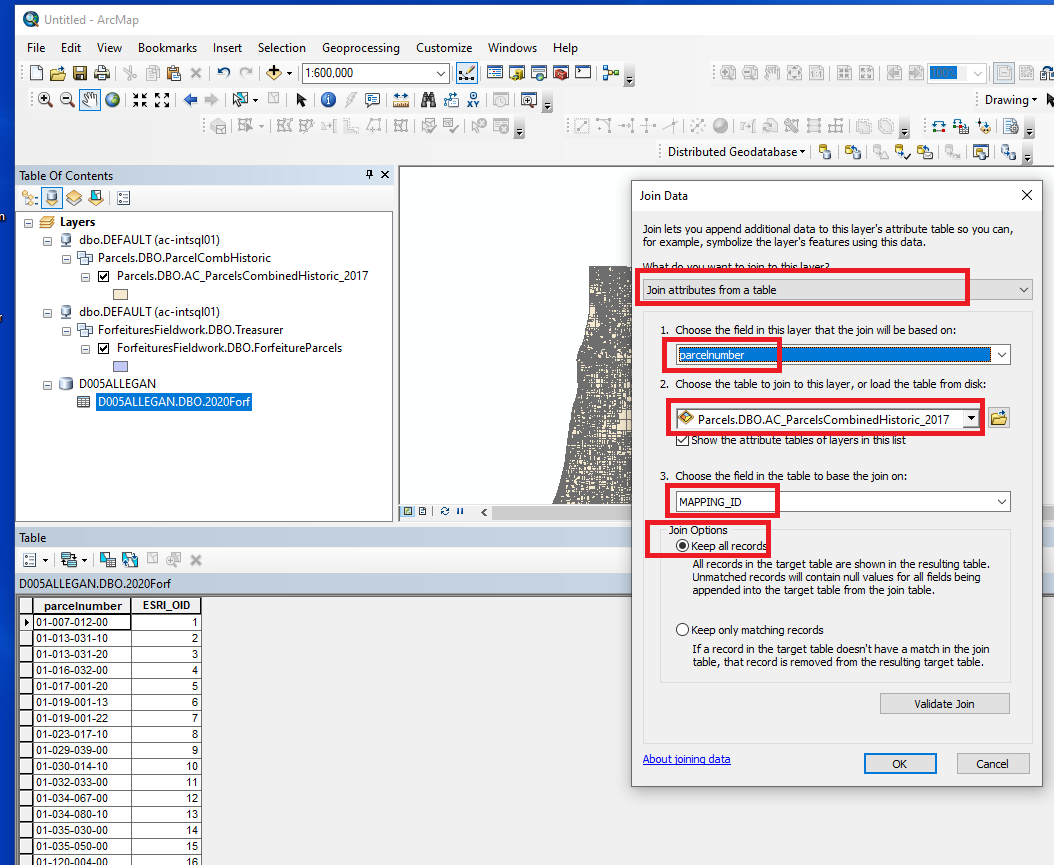
\includegraphics[width=1\textwidth]{joinToForfTable.PNG}
  \caption{Join to Forfeiture Table}
  \end{figure}
  \clearpage



  %\begin{itemize}
  \item {Select any parcels missing spatial data}

  %\end{itemize}

 % \vspace{.25in}

    %
    % Single Figure No Wrap
    %
  \begin{figure}[h!]
  \centering
      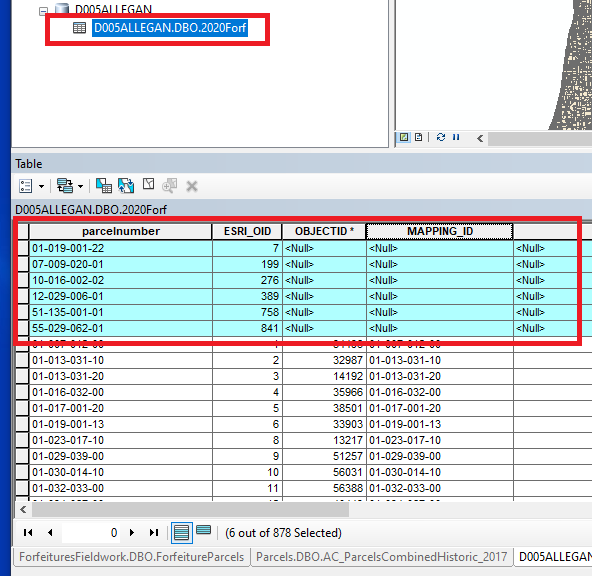
\includegraphics[width=.65\textwidth]{selectForMissingSpatial.PNG}
  \caption{Select for Missing Spatial}
  \end{figure}

  %\begin{itemize}
  \item {Export Parcels missing spatial to a table in the GDB}

  \end{itemize}


  \begin{figure}[h!]
  \centering
      \includegraphics[width=.75\textwidth]{exportMissingSpatial.PNG}
  \caption{Export Missing Spatial}
  \end{figure}

  \clearpage
    %
    %

 \paragraph{Create current year Forfeiture dataset}
  \subparagraph{Create Join}
  \vspace{.3in}

 \begin{itemize}

 \item{Create new join to \emph{ACParcelsCombHistoricXXXX} of forfeitures on parcel numbers}

 \end{itemize}

    %
  \vspace{.25in}

    %
    % Single Figure No Wrap
    %
  \begin{figure}[h!]
  \centering
      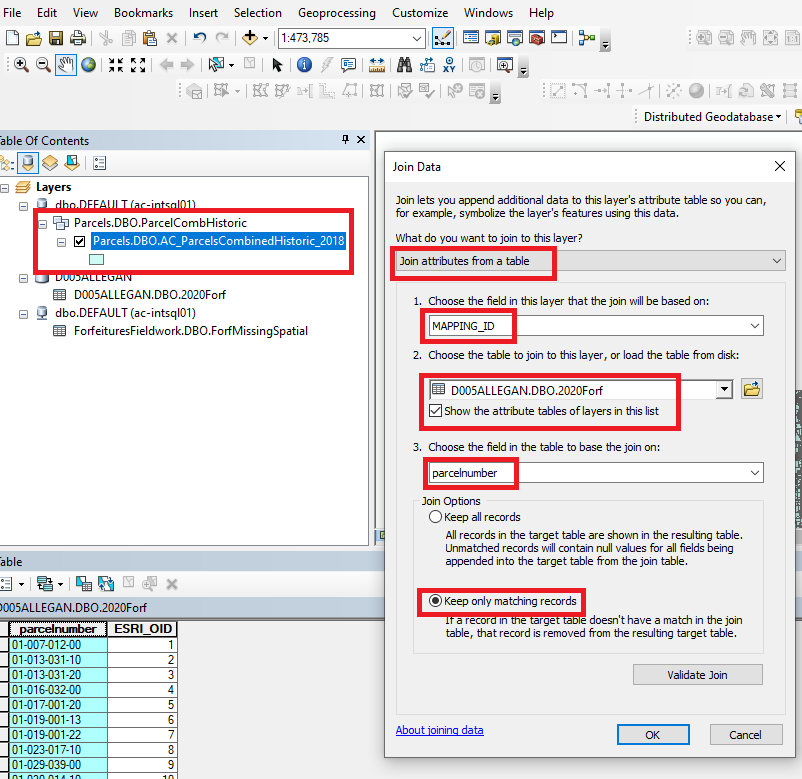
\includegraphics[width=.95\textwidth]{joinToParcelsCombined.PNG}
  \caption{Join Parcels}
  \end{figure}
  \clearpage
    %
    %
  \subparagraph[Export Joined Features]{Export Joined Features to a temp location \texorpdfstring{\\}{}}
    %
  \begin{itemize}
  %\item Right click \ding{212} on joined feature class in TOC and choose export
  \item Right click {{\rtArrow}}  on joined feature class in TOC and choose export
 \end{itemize}
    %
    % Single Figure No Wrap
    %
  \begin{figure}[h!]
  \centering
      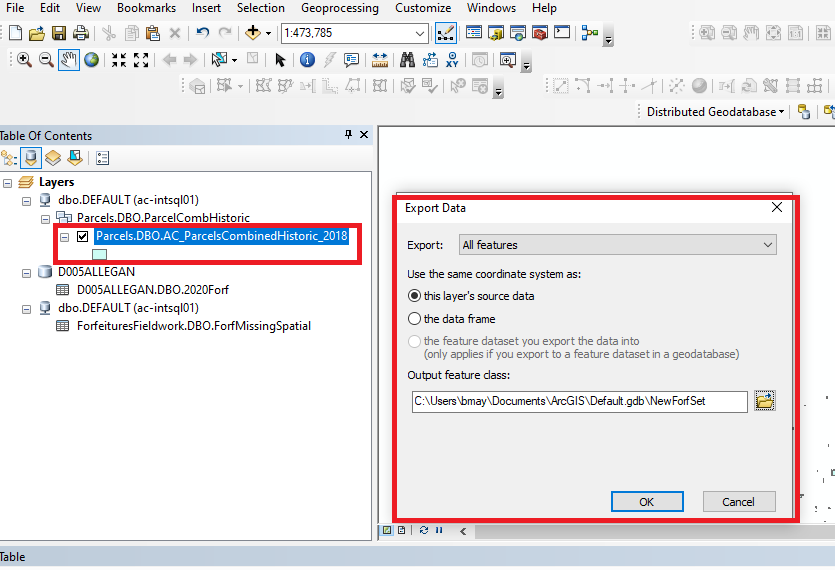
\includegraphics[width=.95\textwidth]{exportJoinedFeatures.png}
  \caption{Export Joined Features}
  \end{figure}
  {\bigbtn choose location and Push \fbox{OK}}
 %\item choose location and Push \fbox{OK}
  %\end{itemize}
  \clearpage
    %
    %
  \subparagraph[Load data to forfeitureParcels]{\Large Load data from temp location to forfeitureParcels}
  %\subparagraph*{}
    %
    % Single Figure No Wrap
    %
  \begin{figure}[h!]
  \centering
      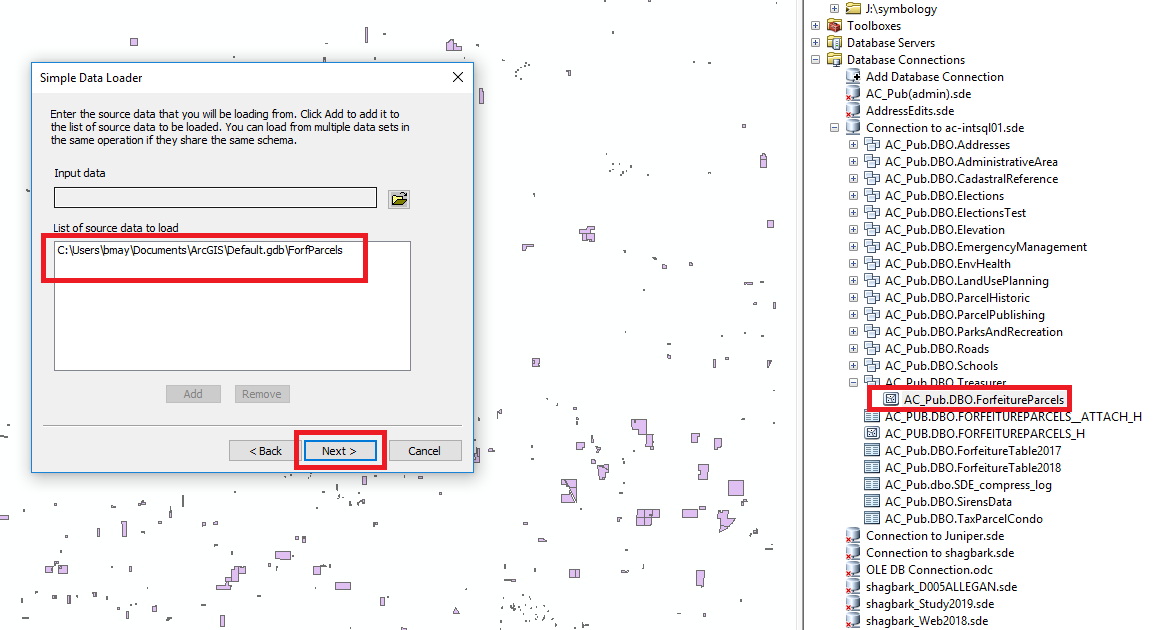
\includegraphics[width=.95\textwidth]{LoadData.PNG}
  \caption{Load Data 1}
  \end{figure}

  {\bigbtn choose features from a temp location}

 \vspace{.2in}

  {\bigbtn Push \fbox{Next}}


    %
    % Single Figure No Wrap
    %
  \begin{figure}[h!]
  \centering
      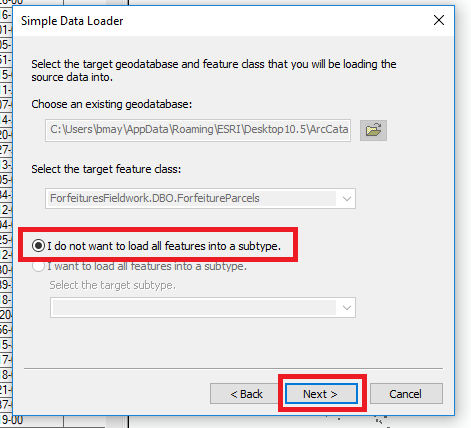
\includegraphics[width=.65\textwidth]{LoadData2.PNG}
  \caption{Load Data 2}
  \end{figure}

 \clearpage

  \paragraph[Match these fields]{\Large Match these fields}

    %
    % Single Figure No Wrap
    %
  \begin{figure}[h!]
  \centering
      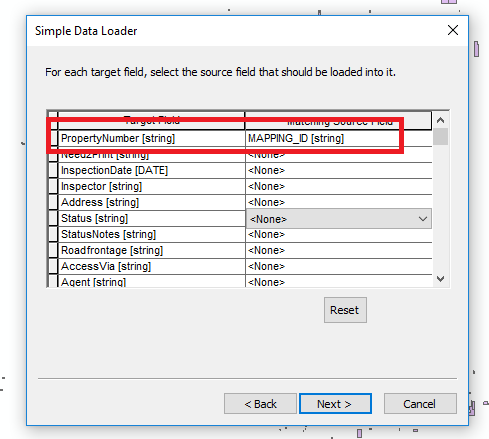
\includegraphics[width=.70\textwidth]{fieldMatch1.PNG}
  \vspace{-.2in}

  \caption{Match Fields 1}
  \end{figure}
  \begin{figure}[h!]
  \centering
      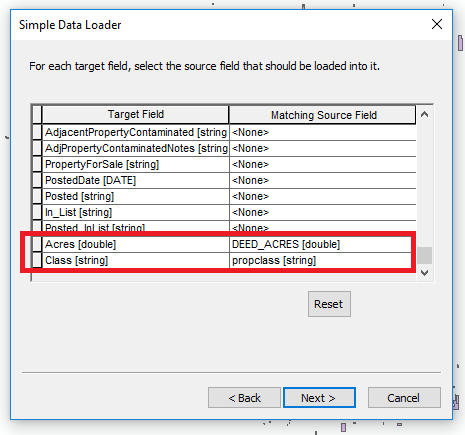
\includegraphics[width=.65\textwidth]{fieldMatch2.PNG}
  \vspace{-.2in}

  \caption{Match Fields 2}
  \end{figure}
  \clearpage
    %
    %
 {\bigbtn Push \fbox{Next}}
 % \paragraph*{\Large Push \fbox{Next}}
    %
    % Single Figure No Wrap
    %
  \begin{figure}[h!]
  \centering
      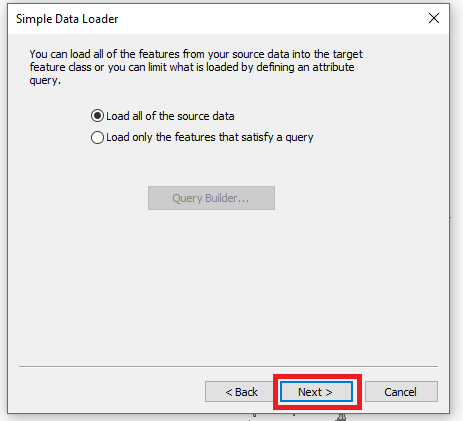
\includegraphics[width=.95\textwidth]{LoadData4.PNG}
  \caption{Load Data 3}
  \end{figure}
    %

 {\bigbtn Push \fbox{Finish}}

    %
  \clearpage
    %
    %


 \paragraph{Calculate Initial Values}


 \subparagraph{Calculate In List value}

 \begin{figure}[h!]
  \centering
      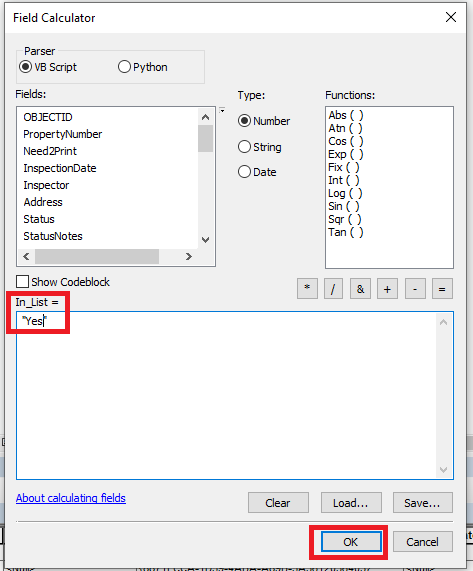
\includegraphics[width=.5\textwidth]{InListToYes.PNG}
  \caption{Calculate In List}
  \end{figure}

 \subparagraph{Calculate Posted Value}

   \begin{figure}[h!]
  \centering
      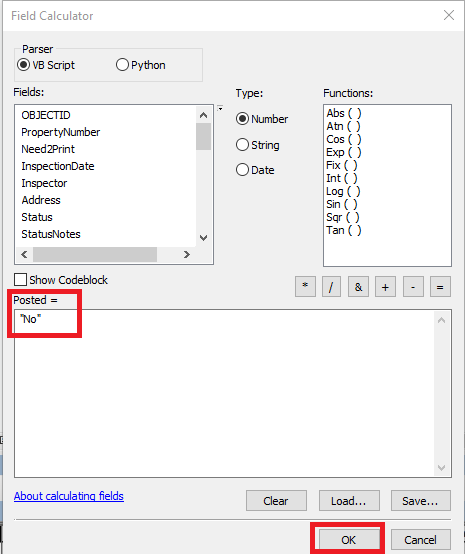
\includegraphics[width=.5\textwidth]{PostedToNo.PNG}
  \caption{Calculated Posted}
  \end{figure}


 \subparagraph{Calculate Posted InList Value}

   \begin{figure}[h!]
  \centering
      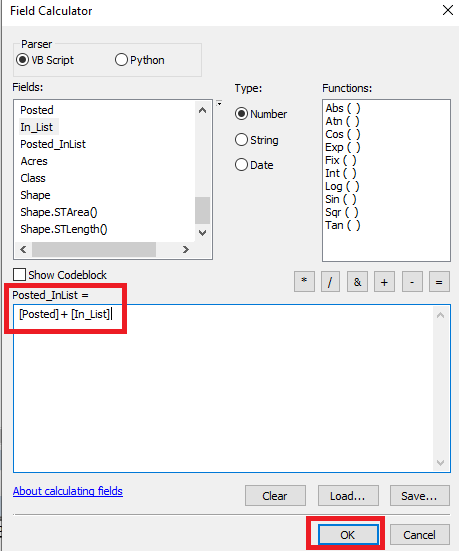
\includegraphics[width=.5\textwidth]{PostedAndInList.PNG}
  \caption{Calculate Posted in List}
  \end{figure}


 \clearpage










  \paragraph{Data Setup}
  \vspace{.2in}

 \subparagraph{Register as versioned and Add Global IDs}


  \vspace{.2in}

  \noindent{\large Right Click {\rtArrow} Manage {\rtArrow} Register as Versioned}
  \vspace{.2in}

  and
  \vspace{.2in}

  \noindent{\large Right Click {\rtArrow} Manage {\rtArrow} Add Global IDs}
  \vspace{.2in}

    %
    % Single Figure No Wrap
    %
  \begin{figure}[h!]
  \centering
      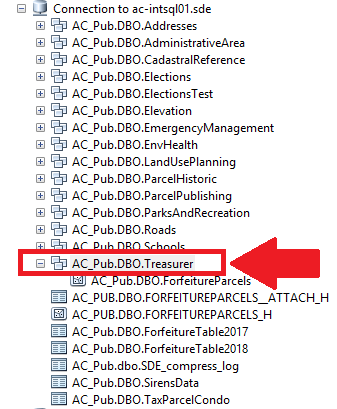
\includegraphics[width=.8\textwidth]{RegisterAsVersioned.PNG}
  \caption{Setup Data}
  \end{figure}
    %
  \clearpage
    %
    %
  \paragraph[Create Attachments]{\Large Create Attachments\texorpdfstring{\\}{}}
 Attachments is for storing the photos for each feature.

  \noindent{\large Right Click {\rtArrow} Manage {\rtArrow} Add Attachments}
  \vspace{.3in}

  \subparagraph*{}
    %
    % Single Figure No Wrap
    %
  \begin{figure}[h!]
  \centering
      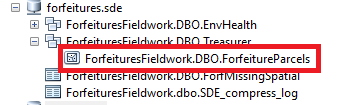
\includegraphics[width=.8\textwidth]{createAttachments.PNG}
  \caption{Create Attachments}
  \end{figure}


   \subparagraph{Calculate Acres in ForfeitureParcels}

 \noindent{\large Right Click {\rtArrow} Acres Column {\rtArrow}Calculate geometry (acres)}

  \clearpage


    %
    %
  \paragraph[Setup Users in ArcGIS]{\Large Setup Users in ArcGIS\texorpdfstring{\\}{}}

  Users that will run Pre and Post processing scripts must be created and given priviliges on Treasurer Feature Data Set.
  \vspace{.35in}

  \noindent For any new users of the geoprocessing tools:

  \vspace{.15in}

  Use the create Database User tool
   \vspace{.15in}

  {\textbf or}

  \vspace{.15in}

 In Catalog {\rtArrow} Right click on ForfeituresFieldwork {\rtArrow} Administration {\rtArrow} Add User

  \vspace{.35in}

    %
    % Single Figure No Wrap
    %
  \begin{figure}[h!]
  \centering
      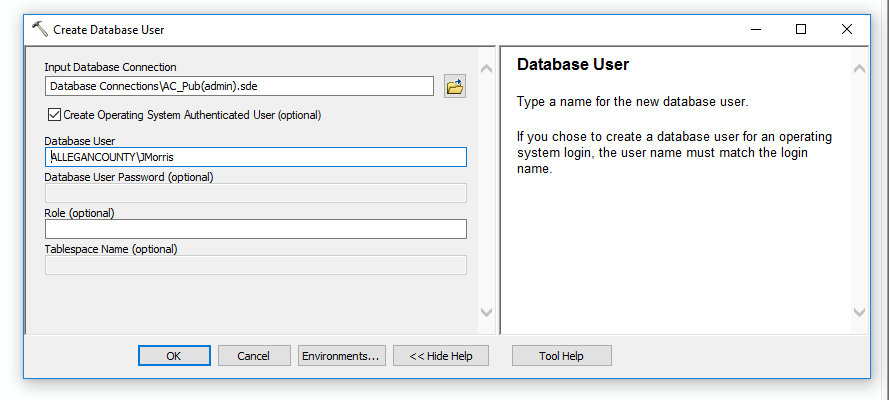
\includegraphics[width=1\textwidth]{addDbUser.png}
  \caption{Add Db User}
  \end{figure}
  \clearpage
    %
    %
  \paragraph[Add New User to Feature Dataset]{\Large Add New User to Feature Dataset\texorpdfstring{\\}{}}
  \vspace{.35in}

  In Catalog, { \rtArrow} right click on Treasurer Feature Data Set
  \vspace{.15in}

  {\rtArrow} Manage { \rtArrow} Priviliges { \rtArrow} Add { \rtArrow} Type new user { \rtArrow}

 \vspace{.25in}

 {\btn Push \fbox{OK}}
  \vspace{.25in}

    %
    % Single Figure No Wrap
    %
  \begin{figure}[h!]
  \centering
      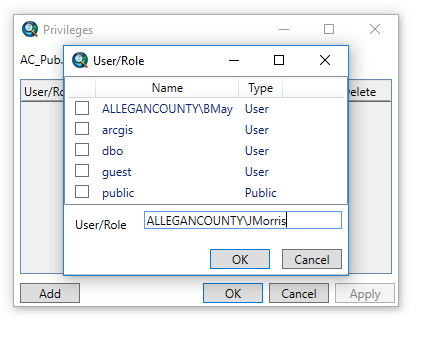
\includegraphics[width=.9\textwidth]{AddFdsUser.png}
  \caption{Add Feature Dataset User}
  \end{figure}
  \clearpage
    %
    %
  \paragraph[Extend Priviliges for New User]{\Large Extend Priviliges for New User\texorpdfstring{\\}{}}
  \vspace{.5in}

  In Catalog {\rtArrow} right click on Treasurer FDS {\rtArrow} Manage {\rtArrow} Priviliges {\rtArrow} check boxes
  \vspace{.5in}

    %
    % Single Figure No Wrap
    %
  \begin{figure}[h!]
  \centering
      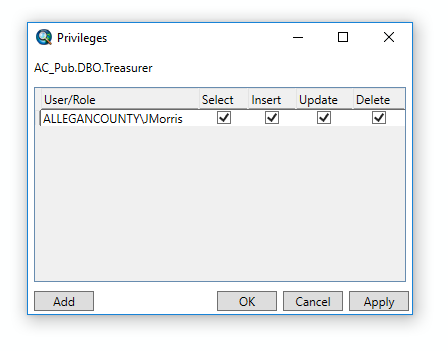
\includegraphics[width=.9\textwidth]{AddFdsUserPriviliges.png}
  \caption{Extend Feature Dataset Priviliges}
  \end{figure}
  \clearpage
    %
    %
 \paragraph{Portal Setup}

 \subparagraph{Setup Users in Portal for ArcGIS}
  \vspace{.5in}

  \noindent Users that will use the Collector for ArcGIS must have profiles added to and managed in the Allegan County GIS Portal site.
  \vspace{.5in}

  In Portal, {\rtArrow} \fbox{My Organization}

 \vspace{.2in}

 {\btn Push \fbox{Add Members}}
 %\paragraph*{\Large Push \fbox{Add Members}}

    %
    % Single Figure No Wrap
    %
  \begin{figure}[h!]
  \centering
      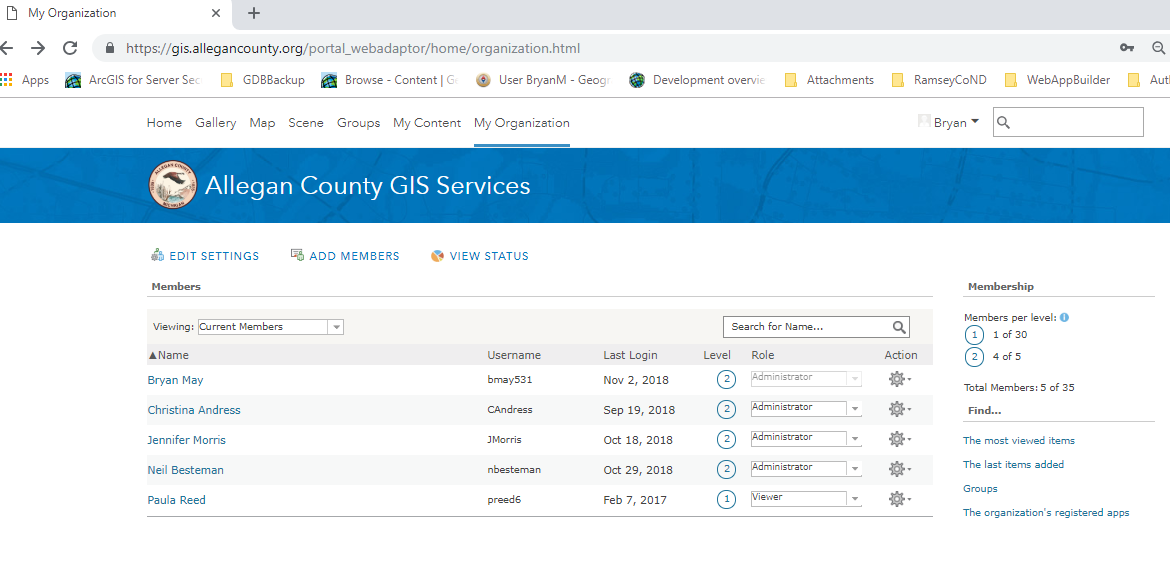
\includegraphics[width=.9\textwidth]{PortalAddUser1.png}
  \caption{Portal Add User 1}
  \end{figure}
  \clearpage
    %
    %

  \subparagraph{Add Members to Portal}

  \vspace{.4in}

  {\Large Select Built in Member {\rtArrow}}
  \vspace{.4in}

    %
    % Single Figure No Wrap
    %
  \begin{figure}[h!]
  \centering
      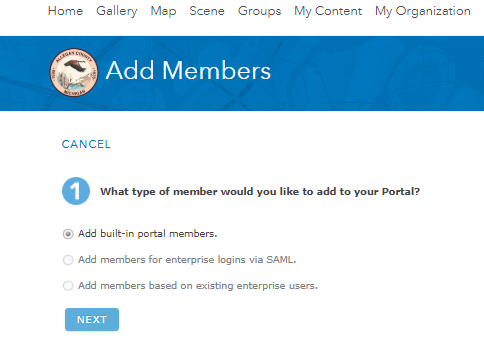
\includegraphics[width=.9\textwidth]{PortalAddUser2.png}
  \caption{Portal Add User 2}
  \end{figure}

 {\bigbtn Push \fbox{Next}}

  \clearpage
    %
    %
  \subparagraph{Enter required info for new member}
    %
  \vspace{.5in}

    %
    % Single Figure No Wrap
    %
  \begin{figure}[h!]
  \centering
      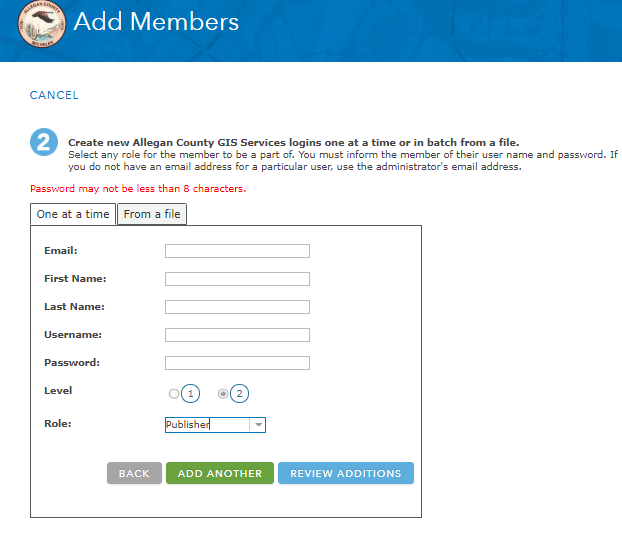
\includegraphics[width=.95\textwidth]{PortalAddUser3.png}
  \caption{Portal Add User 3}
  \end{figure}
  \clearpage
    %
    %
  \subparagraph{Manage Treasurer Group}
  \vspace{.5in}

  In Portal {\rtArrow} Go to groups {\rtArrow} Invite new user to the group
  \vspace{.5in}

    %
    % Single Figure No Wrap
    %
  \begin{figure}[h!]
  \centering
      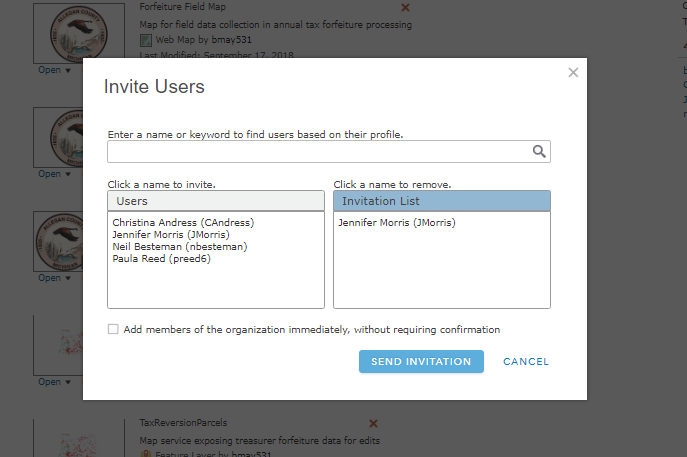
\includegraphics[width=.9\textwidth]{PortalAddUser4.png}
  \caption{Portal Add User 4}
  \end{figure}
  \clearpage
    %
    %
  \subparagraph{Share Portal Content with the group}
  \vspace{.5in}

  \noindent Any content used by the group needs to be shared to the group
  \vspace{.5in}

    %
    % Single Figure No Wrap
    %
  \begin{figure}[h!]
  \centering
      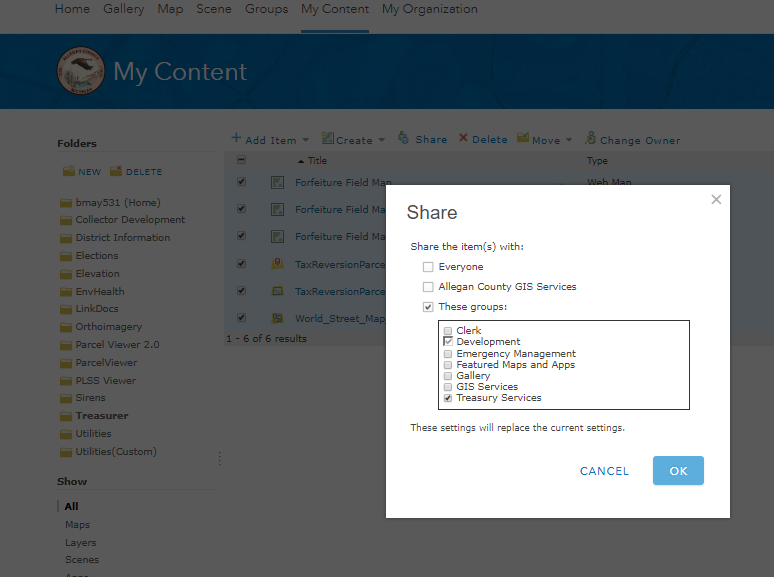
\includegraphics[width=.9\textwidth]{PortalAddUser5.png}
  \caption{Portal AddUser 5}
  \end{figure}
  \clearpage
    %
    %


 \paragraph{Start services and webmap}

 \subparagraph{Find published MXD}

 \begin{figure}[h!]
  \centering
      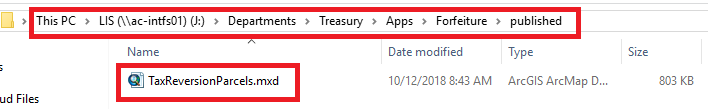
\includegraphics[width=.9\textwidth]{publishedMxd.png}
  \caption{Published Mxd}
  \end{figure}
  \clearpage





 \paragraph{Publish Forfeiture Parcels Map Service}

 \subparagraph{General}
 \begin{figure}[h!]
  \centering
      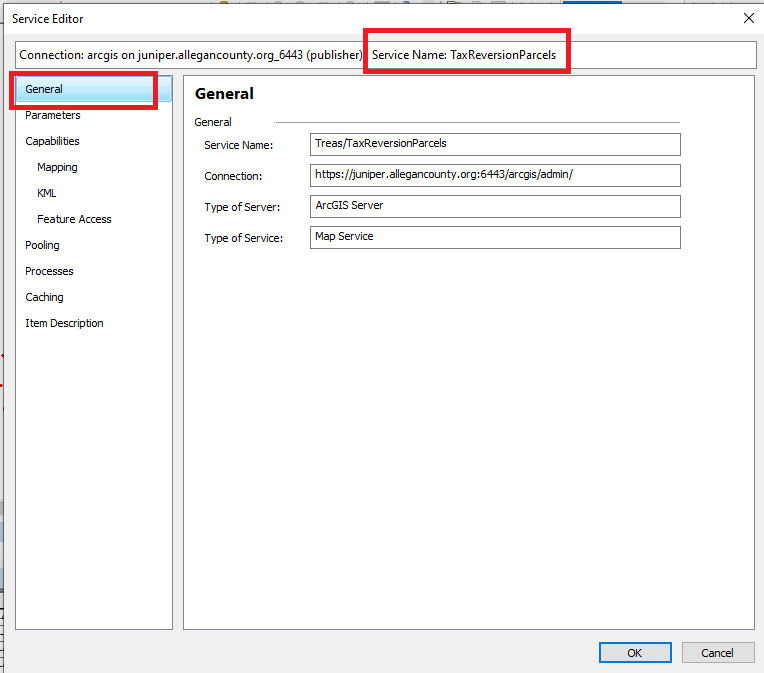
\includegraphics[width=.5\textwidth]{General.png}
  \caption{General}
  \end{figure}
  %\clearpage

 \subparagraph{Capabilities}
 \begin{figure}[h!]
  \centering
      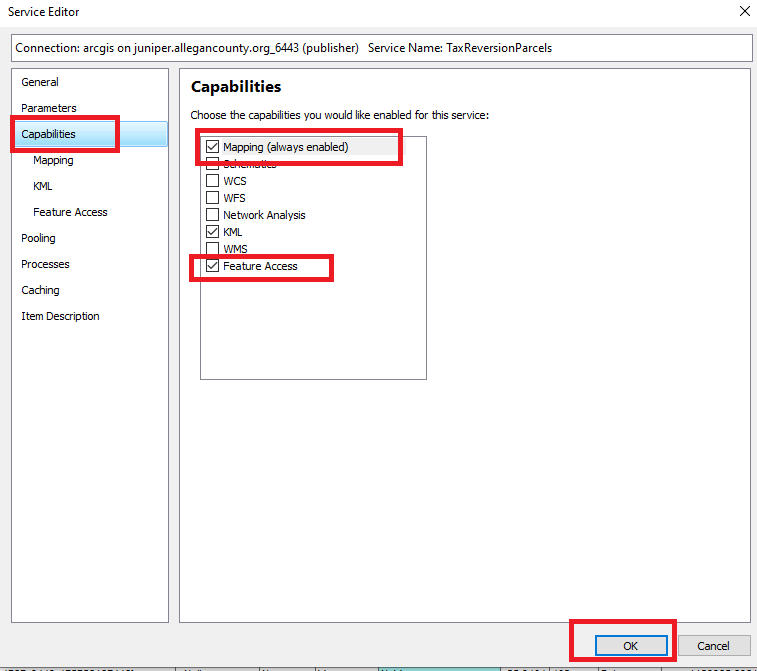
\includegraphics[width=.5\textwidth]{Capabilities.png}
  \caption{Capabilities}
  \end{figure}

  %\clearpage


 \subparagraph{Feature Access}
 \begin{figure}[h!]
  \centering
      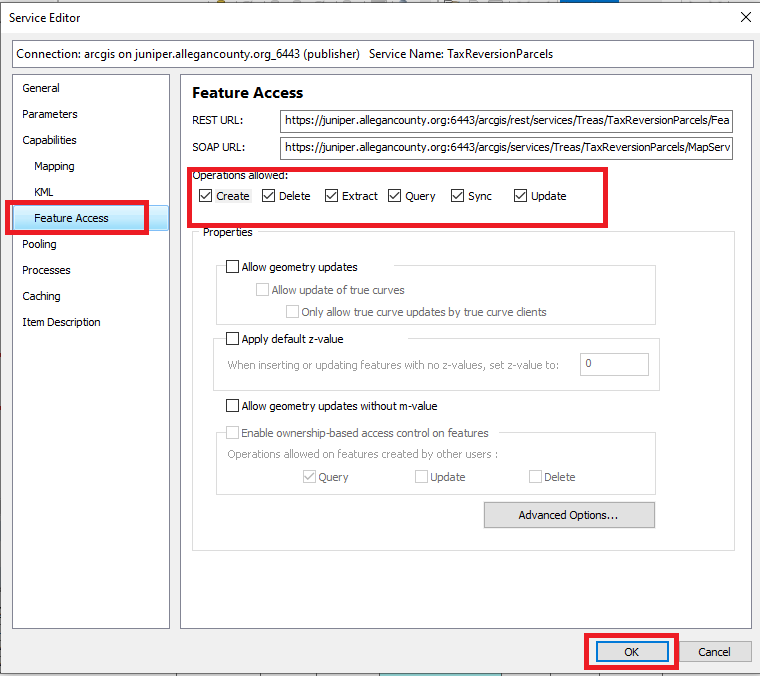
\includegraphics[width=.5\textwidth]{FeatureAccessProperties.png}
  \caption{Feature Access}
  \end{figure}
  \clearpage

 \subparagraph{Publish Service}
 \begin{figure}[h!]
  \centering
      \includegraphics[width=.5\textwidth]{PublishService.png}
  \caption{Publish Service}
  \end{figure}







 \paragraph{Schema Change Procedure}

  \clearpage
    %
    %
  \paragraph[Form Edits Procedure]{\Large Form Edits Procedure}
  

  
  \clearpage
    %
    %
  \subsubsection[User Manual]{\Large User Manual}
    %
  \paragraph{Collection Device Setup}
    %
  \subparagraph{Install Collector for ArcGIS}
	\noindent Available for IOS, Android, and Windows 10\\
	\noindent This workflow supports Collector Classic on IOS
  \begin{itemize}
  \item Get Collector Classic from the App Store
  \end{itemize}
    %
    % Single Figure No Wrap
    %
  \begin{figure}[h!]
  \centering
      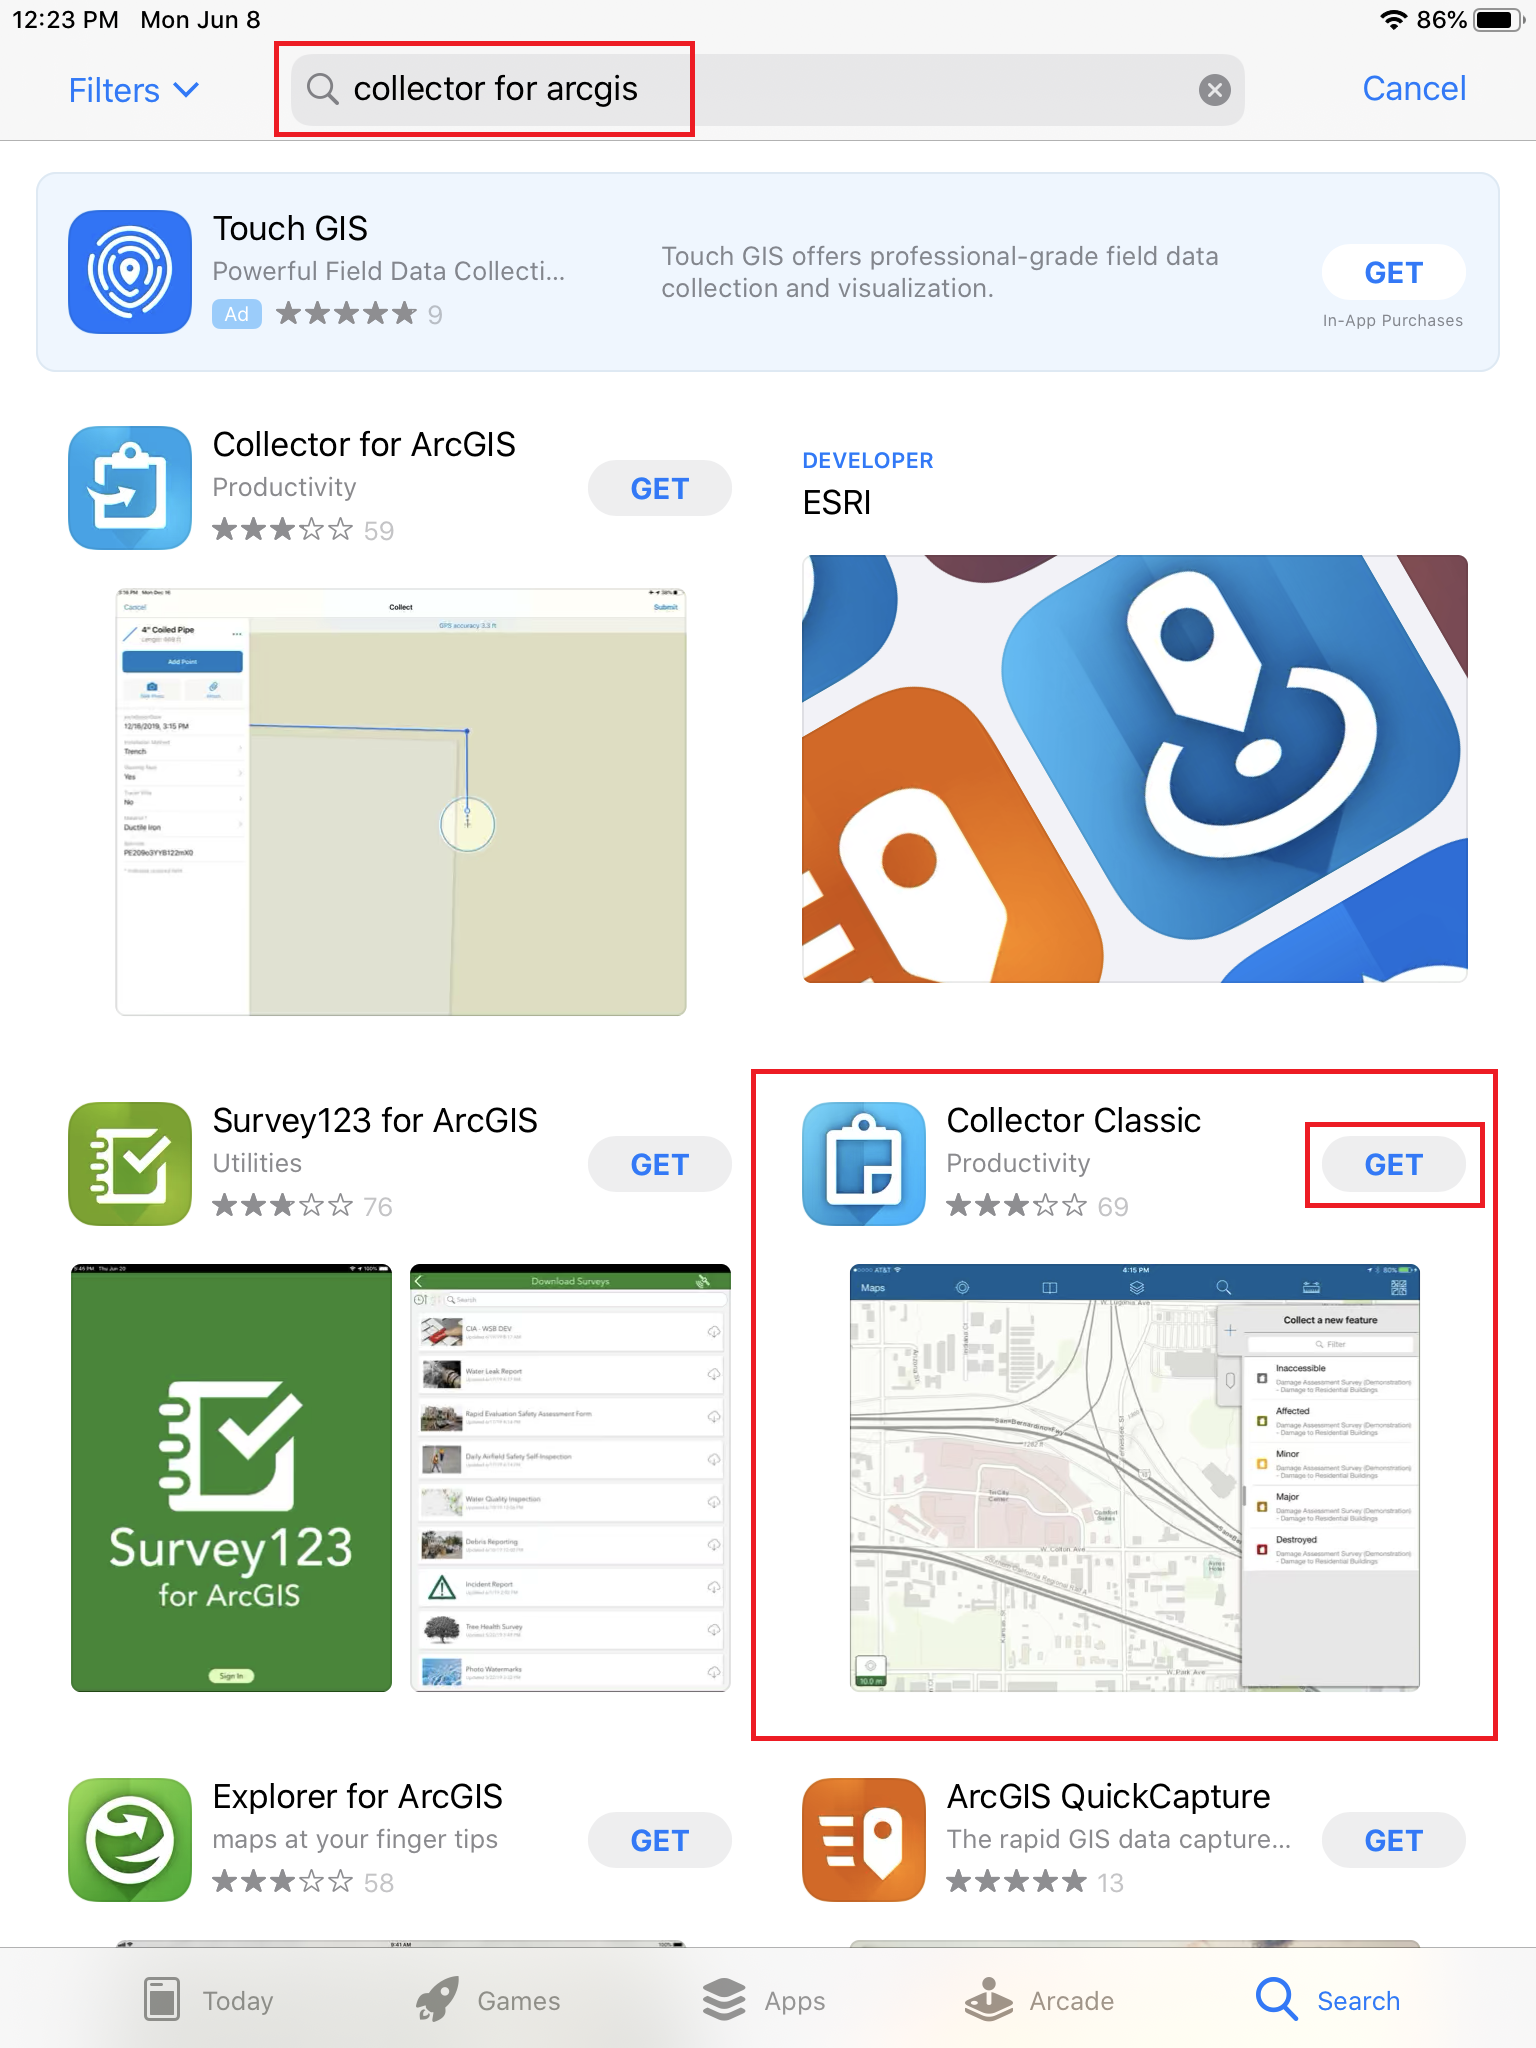
\includegraphics[width=.65\textwidth]{DownloadtheApp.png}
  \caption{Download the App}
  \end{figure}
  \clearpage
    %
    %
  \subparagraph[Configure Collector]{\Large Configure Collector}
    %
    % Two Figures Wrapped
    %
  \begin{wrapfigure}{r}{0.5\textwidth}
  \centering
  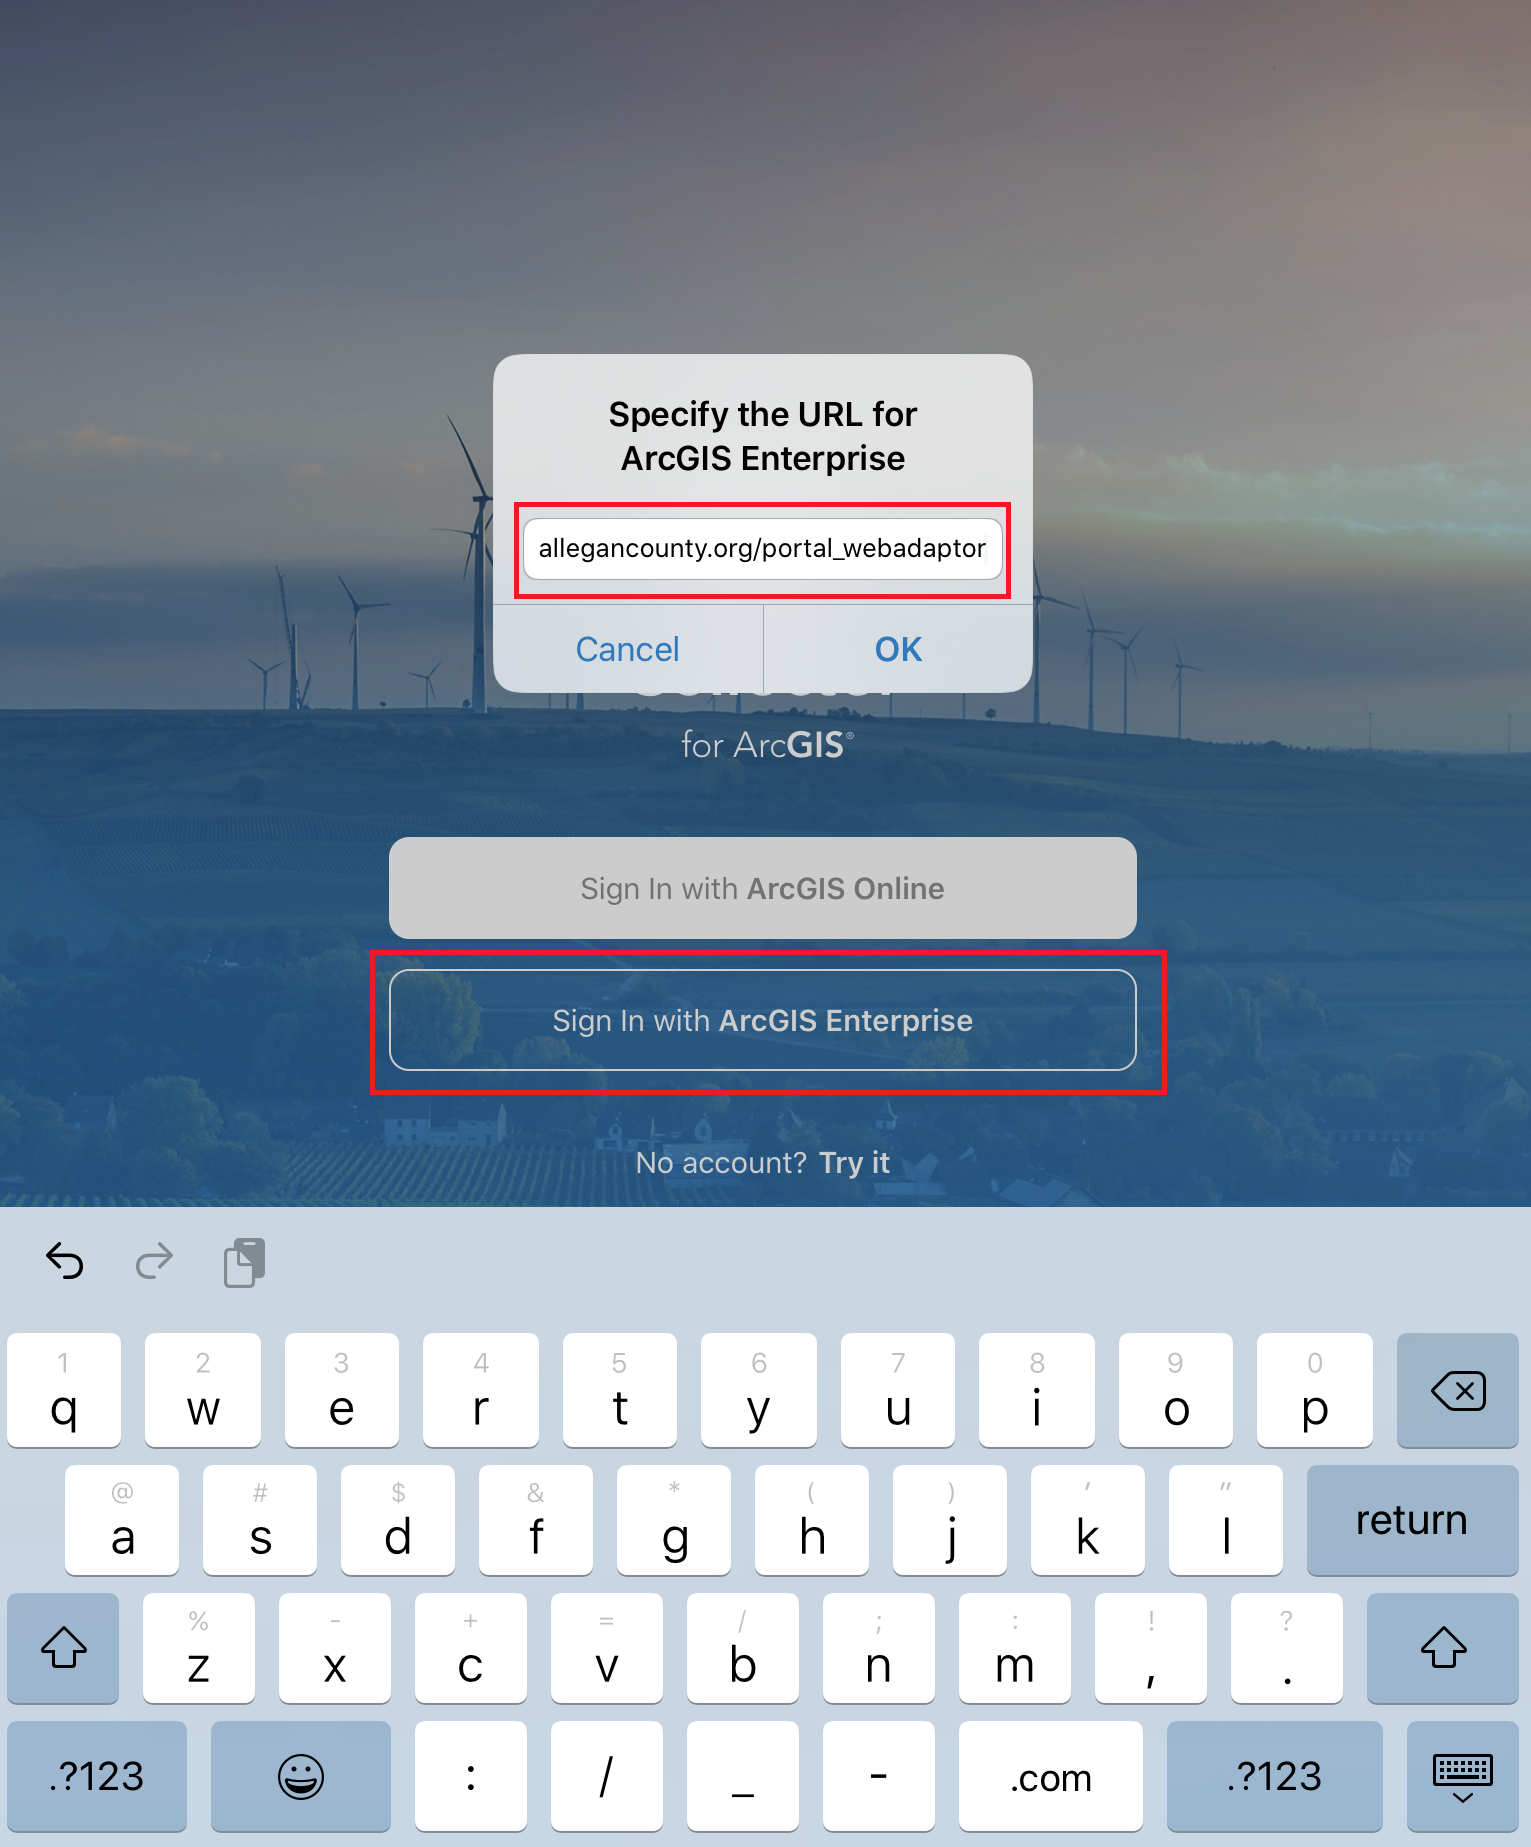
\includegraphics[width=.45\textwidth]{CollectorConnection}
  \caption{Collector Connection}

  \HRule \\[.4cm] % Horizontal Line added
  \vspace{.1in}

      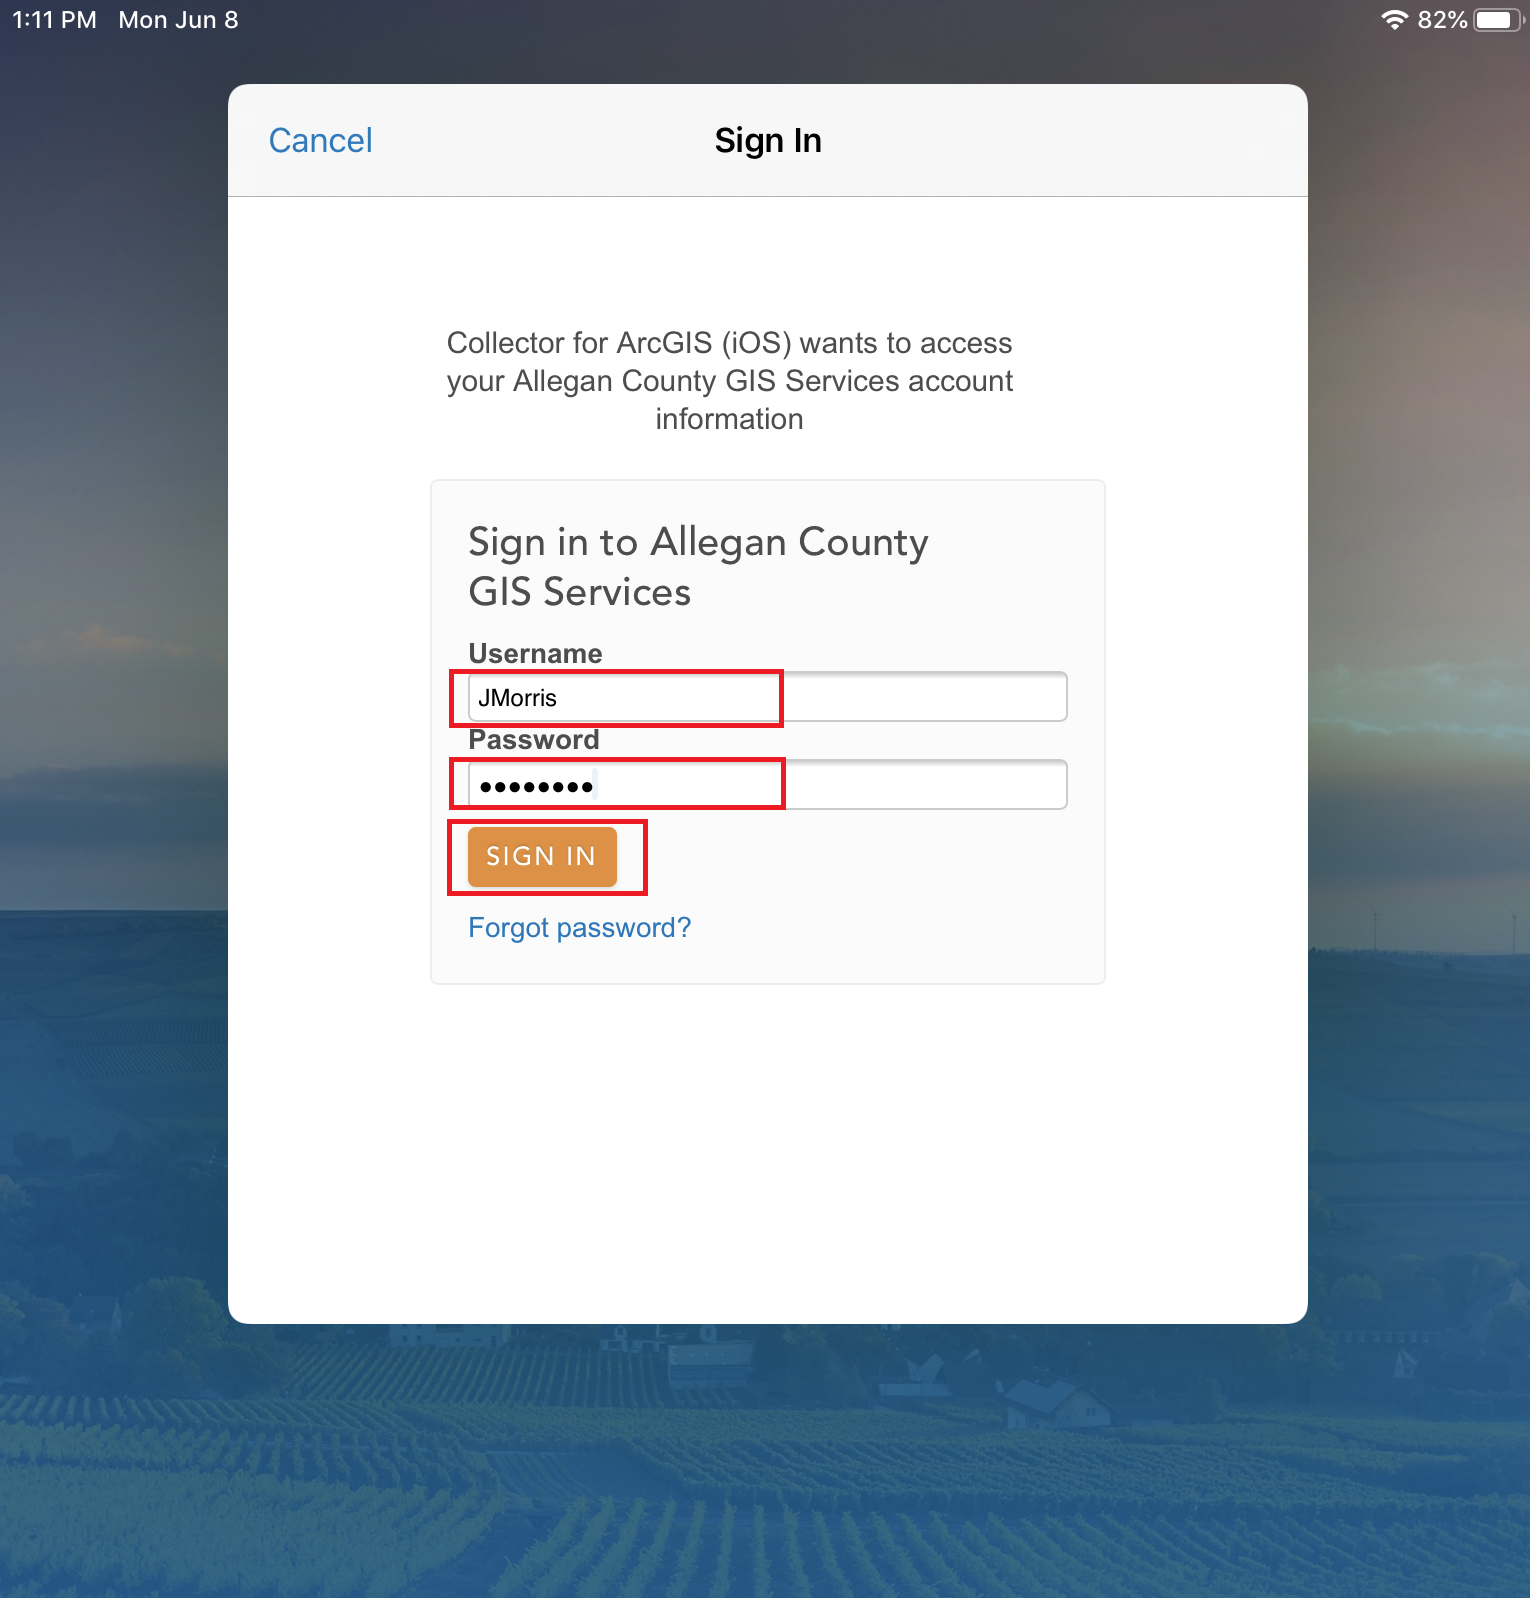
\includegraphics[width=.45\textwidth]{EnterCredentials.png}
  \vspace{-.1in}

  \caption{Enter Credentials}
  \end{wrapfigure}

  %\vspace{.25in}
  Choose\\
  \noindent \textbf{Sign in with ArcGIS Enterprise}
  
 \vspace{.25in}
  
 for \textbf{Organization Website}, Type:
  
 \vspace{.1in}

 \begin{verbatim}

 https://gis.allegancounty.org/
 portal_webadaptor

 \end{verbatim}

  \vspace{.25in}

 \noindent {\btn Push \fbox{OK} \lookArrow}
 \vspace{2in}

  \noindent {\Large Enter Credentials}
  \vspace{1in}

 \noindent {\btn Push \fbox{SIGN IN} \lookArrow}

  \clearpage
    %
    %
  \subparagraph[Download the Forfeiture Field Map]{Download the Forfeiture Field Map \texorpdfstring{\\}{}}
    %
  \noindent There are 3 different versions of the map
    %
  \vspace{.05in}

  \begin{itemize}
  \item Forfeiture Field Map
  \item Forfeiture Field Map For Photos
  \item Forfeiture Field Map For Attributes
  \end{itemize}
    %
  \noindent {\scriptsize The cloud with one arrow indicates it is not on the device but is available for offline use}

    %
    % Two Figures Wrapped
    %
  \begin{wrapfigure}{r}{0.6\textwidth}
  \centering
      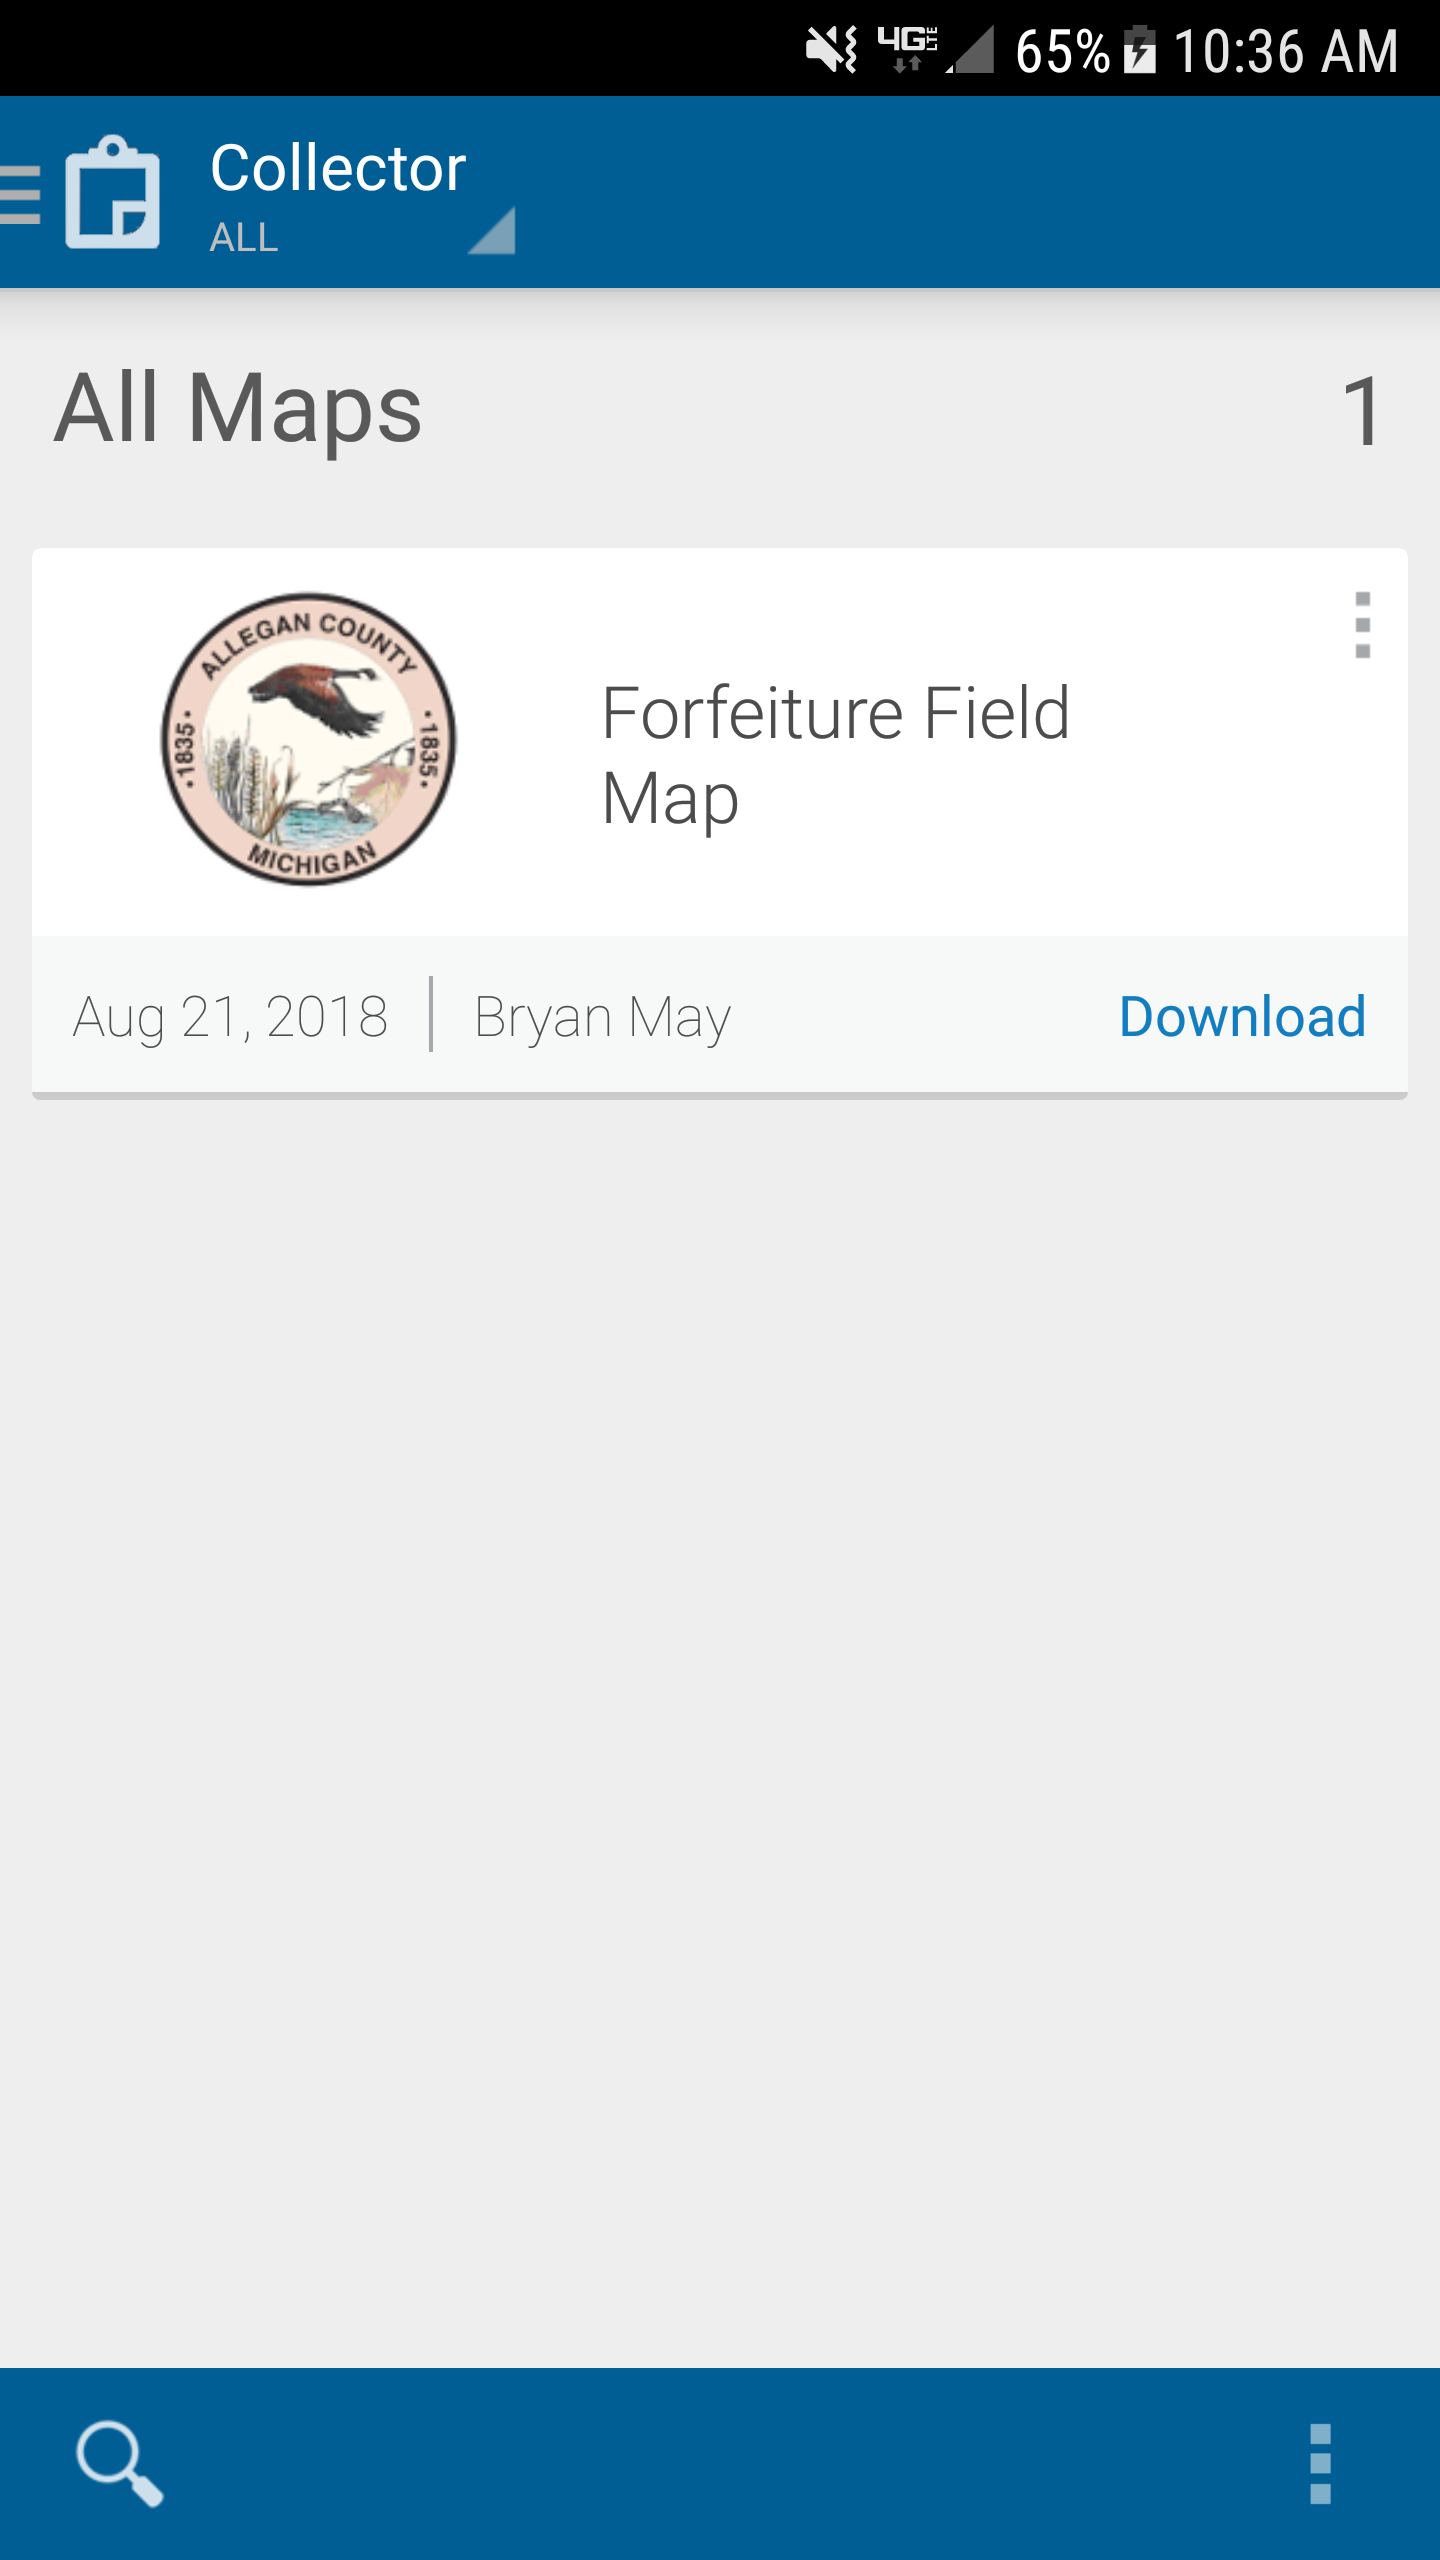
\includegraphics[width=.5\textwidth]{CollectorMapsMenu.png}
  \caption{Collector Maps Menu}
  \end{wrapfigure}
    %
 .
  \vspace{.5in}

  \noindent {\LARGE Choose a Map}
  \vspace{1.75in}

 \noindent {\btn {Push }\fbox{the cloud button}}

  \begin{flushright}
\lookArrow
\end{flushright}
  \clearpage
    %
    %
  \begin{wrapfigure}{r}{0.6\textwidth}
  \centering
      \includegraphics[width=.5\textwidth]{chooseWorkAreaLarge.png}
  \caption{Choose Work Area (large)}
  
  \HRule \\[.4cm] % Horizontal Line added
  \vspace{.1in}

      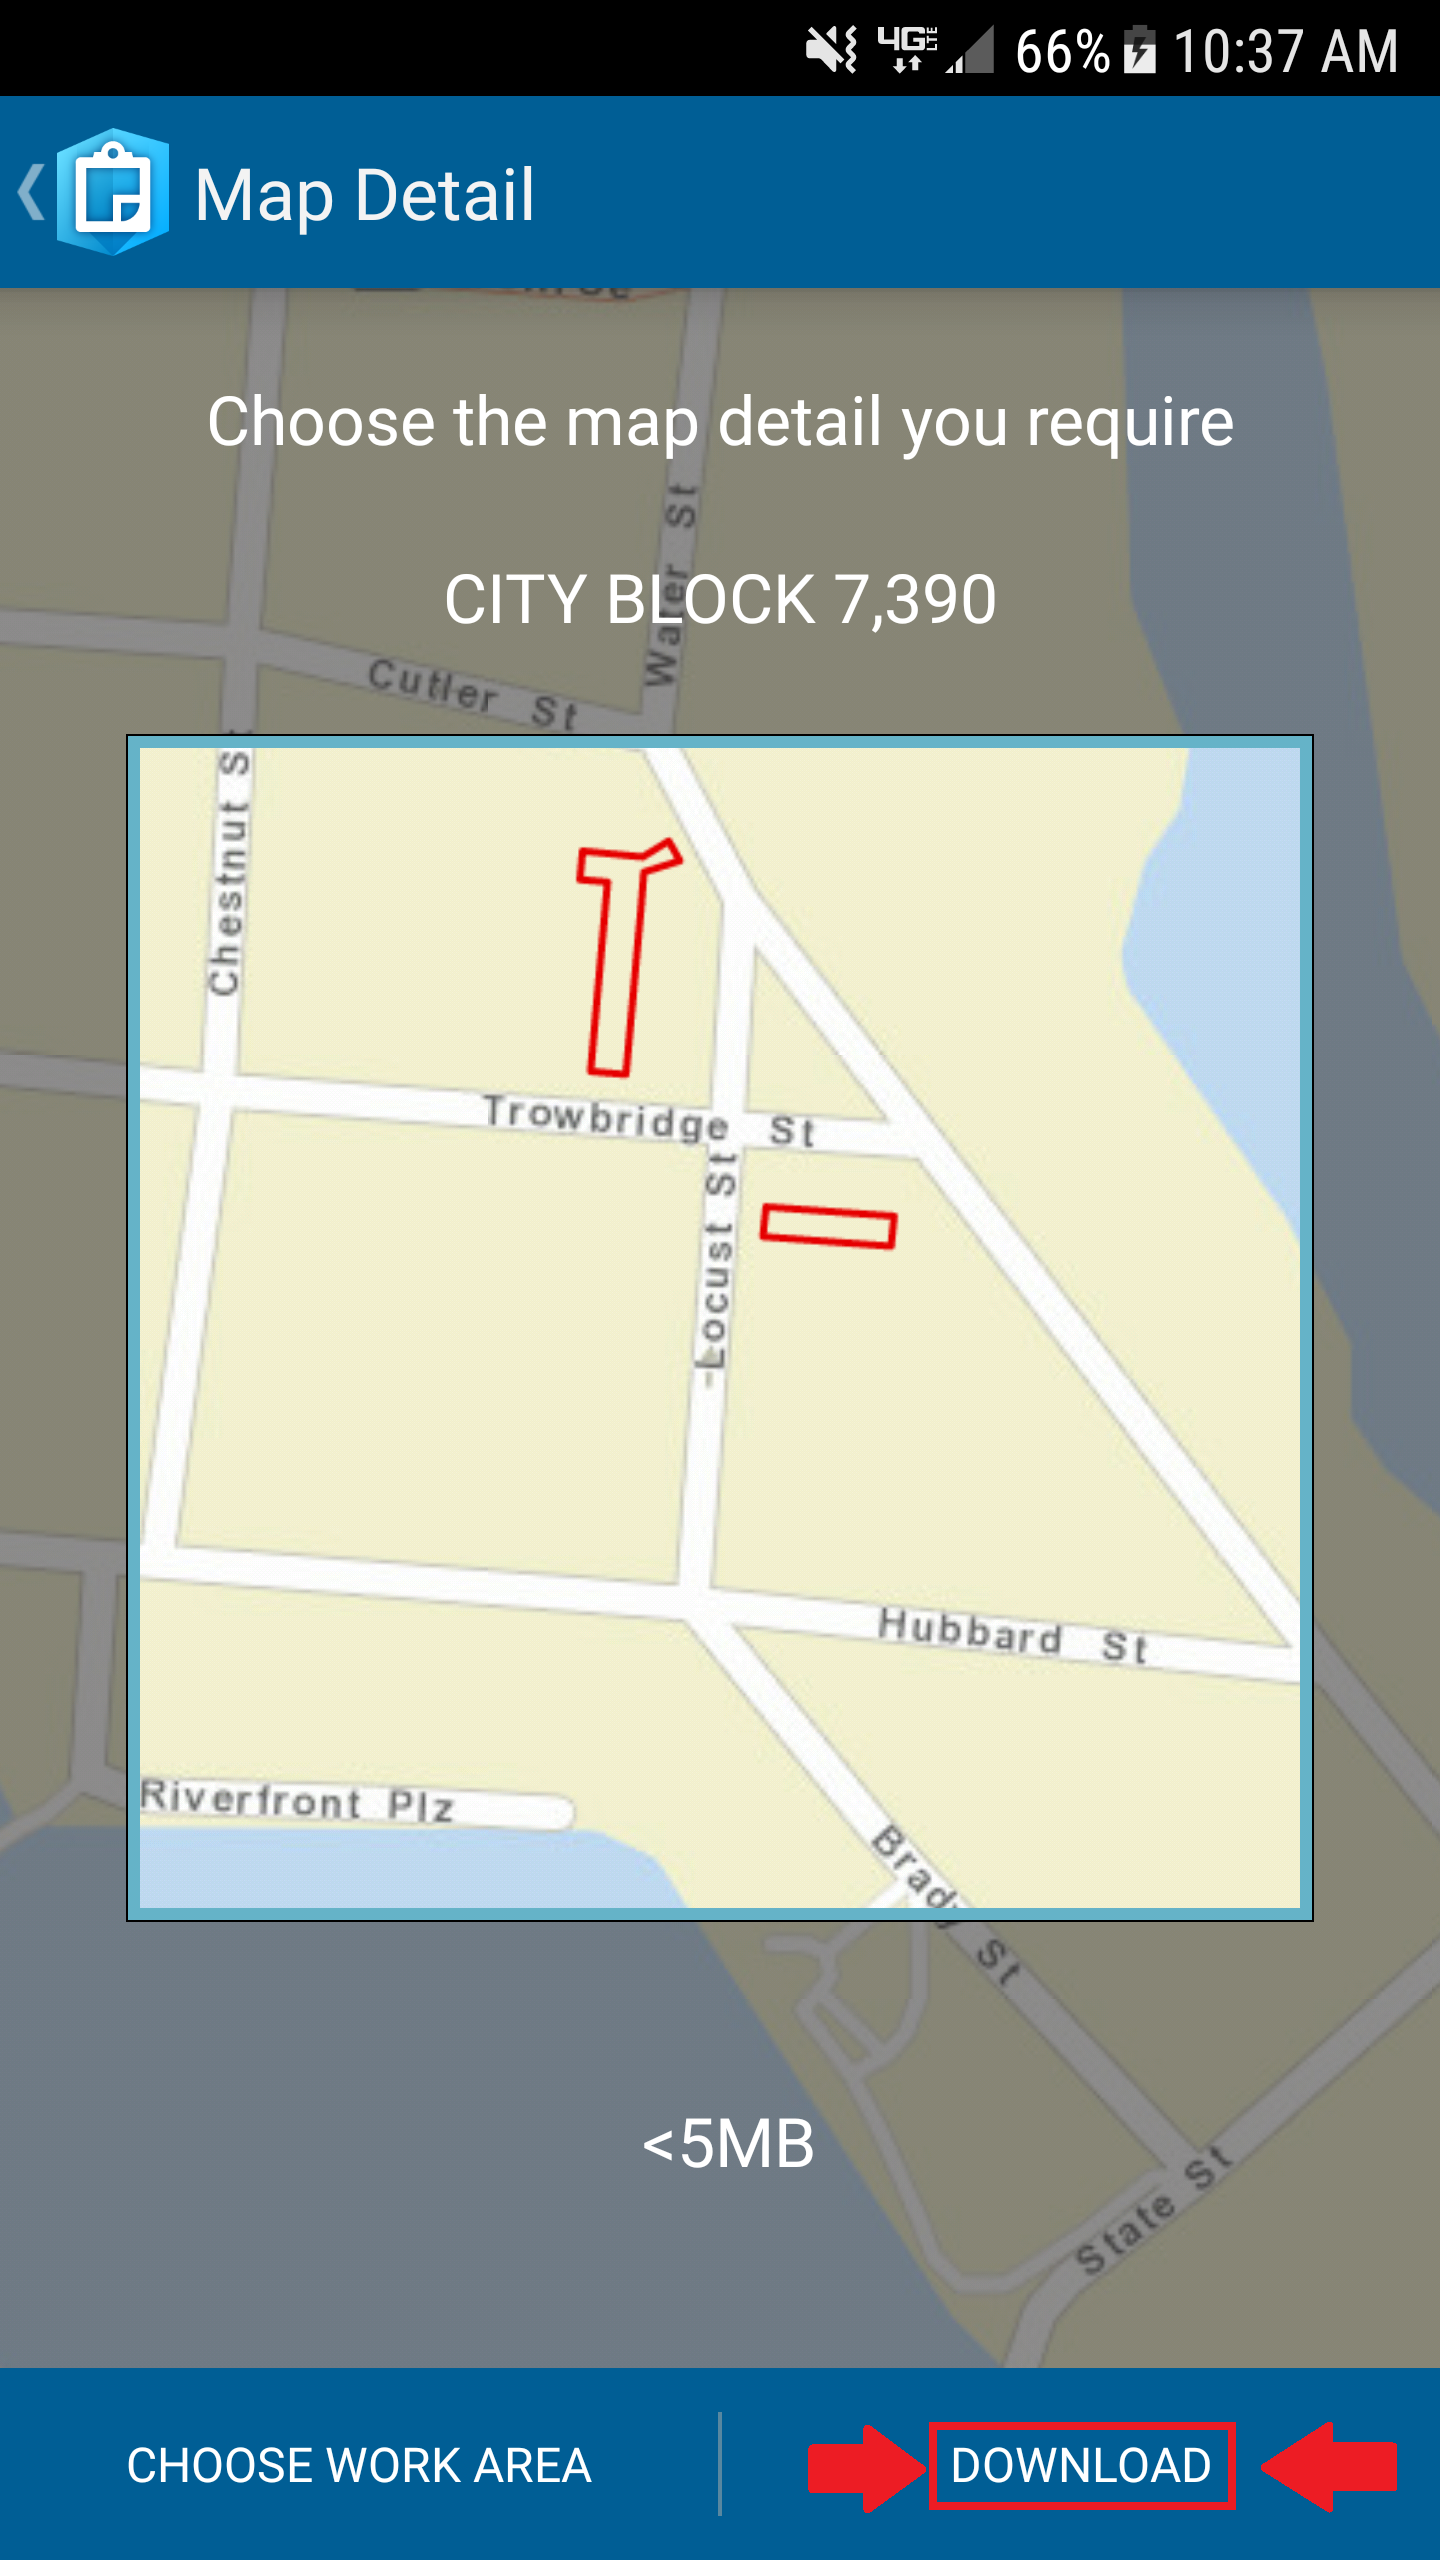
\includegraphics[width=.45\textwidth]{ChooseMapDetail.png}
  \caption{Choose Map Detail}
  \vspace{-.1in}

  \end{wrapfigure}

  \noindent {\Large Specify work area}
  \vspace{1in}

  \noindent {\btn\fbox{Define Area of Interest}}\\
  
  \begin{flushright}
\lookArrow
\end{flushright}
    %
  \vspace{.1in}

  \noindent {\tiny Note that a larger area takes longer to download but the basemap only needs to be downloaded once}
    %
    %
  \vspace{2in}
  
  
  \noindent {\btn Push \fbox{Map Detail}}
  \vspace{.25in}
  
\begin{flushright}
\lookArrow
\end{flushright}
  
  \noindent Zoom into the level of detail desired
    
 \vspace{1in}
  
  {\btn\fbox{Push Download} \lookArrow}
  
  \clearpage
  
    %
    %
 \paragraph{Preprocessing Routine}
    %

 \vspace{.2in}

 Each day the data must be prepared by executing the tool:
 \vspace{.2in}

 \textbf{1. Preprocess}

 \vspace{.2in}

  \subparagraph*{What the tool does:}
  \vspace{.15in}

    %
  \begin{itemize}
  \item Exports current forfeiture list from BSA
    %
  \item Updates webmap layers with results from BSA export
  \end{itemize}
    %
  To use the preprocess tool:
    %
 \vspace{.15in}

 \noindent In the Catalog window, navigate to:
    %
  %{\scriptsize\path{J:\Departments\Treasury\Apps\Forfeiture\processing\ForfeitureToolbox.tbx}}

 %\noindent \href{J:\Departments\Treasury\Apps\Forfeiture\processing\ForfeitureToolbox.tbx}{J:\Departments\Treasury\Apps\Forfeiture\processing\ForfeitureToolbox.tbx}
 \noindent \textcolor{HyperlinkBlue1}{\scriptsize\path{J:\Departments\Treasury\Apps\Forfeiture\processing\ForfeitureToolbox.tbx}}
  %
  %
  \begin{wrapfigure}{r}{0.5\textwidth}
  \centering
      \includegraphics[width=.45\textwidth]{preprocess.png}
  \vspace{-.1in}

  \caption{Processing Tools}
  \end{wrapfigure}
  .
  \vspace{2in}

 \noindent{\bigbtn\fbox{Open the toolbox}  \lookArrow}
  \vspace{.5in}

 \noindent{\bigbtn\fbox{1.Preprocess} \lookArrow}
 
 \noindent Double click on the tool


 \clearpage


 \paragraph*{Preprocessing Routine Cont.}
    %

  \subparagraph{Execute the Preprocess Tool}
  \vspace{.15in}

    %
  \begin{itemize}
    %
  \item Set parameters of the tool
  \end{itemize}
    %
 
 \vspace{.15in}

 \noindent In the tool, navigate to:
    %
  \noindent \textcolor{HyperlinkBlue1}{\scriptsize\path{J:\Departments\Treasury\Apps\Forfeiture\source\Forfeitures.csv}}
  % 
  %
 
  \begin{figure}[h!]
  \centering
      \includegraphics[width=.75\textwidth]{bsaExport.png}
  \vspace{-.1in}

  \caption{Select BSA Export}
 \end{figure}
 
 {\bigbtn Push \fbox{Open}  \lookArrow} 

 {\bigbtn Push \fbox{OK} on the tool to execute  \lookArrow} 

\clearpage


\subparagraph*{Fieldwork data is updated from BSA}




  \begin{figure}[h!]

\centering
     \includegraphics[width=.9\textwidth]{preprocessRunning.png}
\caption{Preprocess Running}
  \vspace{.5in}
 
  \HRule \\[.4cm] % Horizontal Line added
  \vspace{.5in}
    
     \includegraphics[width=.9\textwidth]{preprocessCompleted.png}
\caption{Preprocess Completed}
 \end{figure}


\noindent Now that the fieldwork data is updated, mobile devices must be updated. 



\clearpage
  %
  %


 \subparagraph{Synchronize the Forfeiture Field Map}
  \vspace{.2in}
  
\noindent On the fieldwork devices:

   % Two Figures Wrapped
   %
 \begin{wrapfigure}{r}{0.6\textwidth}
 \centering
     \includegraphics[width=.5\textwidth]{MapToSync}
 \vspace{-.2in}
 
 \caption{Map Downloaded}
 \vspace{-.1in}

 \HRule \\[.4cm] % Horizontal Line added
 \vspace{-.1in}

     \includegraphics[width=.5\textwidth]{mapSynchronized}
 \vspace{-.2in}

 \caption{Map Synchronized}
 \end{wrapfigure}
 \vspace{.5in}
 
{\smallbtn Note the date and time}
 \vspace{.5in}

{\bigbtn Push \fbox{Sync}  \lookArrow}

 \vspace{4in}

 {\smallbtn Note the date and time}
 \vspace{1in}

\noindent{\smallbtn If date has been updated then map is now synchronized}

 \clearpage
   %
   %

 \paragraph{Field Data Collection}
 
 \subparagraph{Data Entry Details}

 Attributes are of three entry types:
 \begin{itemize}
 \item Prefilled {\scriptsize (in preprocessing)}
 %\item Autofill
 \item Dropdown
 \item Text box
 \end{itemize}
   %
 \vspace{1in}

 \subparagraph{Mobile Device Summary}

 For each site visited,

 \begin{itemize}
 \item Select the desired parcel
 \item Push \fbox{Edit}
 \item Collect attributes or photos
 \item Update parcel on device
 \end{itemize}

 \clearpage


 \subparagraph{Device 1 Field Operation}

   %
   % Two Figures Wrapped
   %
 \begin{wrapfigure}{r}{0.5\textwidth}
 \centering
     \includegraphics[width=.45\textwidth]{selectParcel.png}
 \vspace{-.1in}
 
 \caption {Select a Parcel}
   %
 \vspace{.1in}

 \HRule \\[.4cm] % Horizontal Line added
 \vspace{.1in}

 \centering
     \includegraphics[width=.45\textwidth]{editParcel.png}
     \vspace{-.1in}
     
 \caption{Edit Parcel}
 \end{wrapfigure}
   %
 .
   %
 \vspace{2in}

 \noindent{\bigbtn\fbox{Select a Parcel} \lookArrow}
 \vspace{3.5in}

 \noindent{\bigbtn\fbox{Edit} \lookArrow}
 \clearpage
   %
   %
 \subparagraph*{Device 1 Field Operation}
   %
   % Two Figures Wrapped
   %
 \begin{wrapfigure}{r}{0.6\textwidth}
 \centering
     \includegraphics[width=.5\textwidth]{printToday.png}
 \caption {Print Today}
 \vspace{.05in}

 \HRule \\[.4cm] % Horizontal Line added
 \vspace{.05in}

     \includegraphics[width=.5\textwidth]{inspectionDate.png}
 \caption{Enter Date}
 
 \end{wrapfigure}
 %.

 {\footnotesize (cont.)}
 \vspace{.8in}

 \noindent{\bigbtn\fbox{Print Today} \lookArrow}
 \vspace{.5in}
 
 \noindent This will tag parcel for report production in postprocessing
 \vspace{4in}

 \noindent{\bigbtn\fbox{Inspection Date} \lookArrow}


 \clearpage



\subparagraph*{Device 1 Field Operation}
   %
   % One Figures Wrapped
   %
 \begin{wrapfigure}{r}{0.6\textwidth}
 \centering
     \includegraphics[width=.5\textwidth]{selectInspector.png}
\caption{Select Inspector}

 \vspace{3in}

 \end{wrapfigure}
  

 {\footnotesize (cont.)}
 \vspace{.8in}
 
 \noindent{\bigbtn\fbox{Inspector} \lookArrow}

\clearpage

 \subparagraph*{Device 1 Field Operation}
   %
   % Two Figures Wrapped
   %
 \begin{wrapfigure}{r}{0.6\textwidth}
 \centering
     \includegraphics[width=.5\textwidth]{status.png}
 \caption {Occupied or Not}
 \vspace{.05in}

 \HRule \\[.4cm] % Horizontal Line added
 \vspace{.05in}

     \includegraphics[width=.5\textwidth]{statusNotes.png}
 \caption{Enter Text}
 \end{wrapfigure}
 

 {\footnotesize (cont.)}
 \vspace{.8in}

 \noindent{\bigbtn\fbox{Status} \lookArrow}

 \vspace{4in}

 \noindent{\bigbtn\fbox{Status Notes} \lookArrow}

 \clearpage
   %
 
 
  \subparagraph*{Device 1 Field Operation}
   %
   % Two Figures Wrapped
   %
 \begin{wrapfigure}{r}{0.6\textwidth}
 \centering
     \includegraphics[width=.4\textwidth]{roadFrontage.png}
     \vspace{-.1in}
     
 \caption{Road Frontage} 
 
 \vspace{.05in}

 \HRule \\[.4cm] % Horizontal Line added
 \vspace{.05in}
 
    \includegraphics[width=.4\textwidth]{accessVia.png}
 \caption {Enter Text}
 
 \end{wrapfigure}
 
 {\footnotesize (cont.)}
 
 
  \vspace{.5in}

 \noindent{\bigbtn\fbox{Road Frontage} \lookArrow}
 
 \vspace{4in}

 \noindent{\bigbtn\fbox{Access Via} \lookArrow}
 
 \clearpage
 
   %
 \subparagraph*{Device 1 Field Operation}
   %
   % Two Figures Wrapped
   %
 \begin{wrapfigure}{r}{0.6\textwidth}
 \centering
     \includegraphics[width=.4\textwidth]{agent.png}
     \vspace{-.1in}
     
 \caption{Enter Text}
 \vspace{.05in}

 \HRule \\[.4cm] % Horizontal Line added
 \vspace{.05in}

     \includegraphics[width=.4\textwidth]{agentContact.png}
     \vspace{-.1in}
     
 \caption{Enter Text}
 \end{wrapfigure}
 {\footnotesize (cont.)}


 \noindent{\bigbtn\fbox{Agent} \lookArrow}

 \vspace{5.5in}

 \noindent{\bigbtn\fbox{Agent Contact Info} \lookArrow}

 \clearpage


 \subparagraph*{Device 1 Field Operation}
   %
   % Three Figures Wrapped
   %
 \begin{wrapfigure}{r}{0.6\textwidth}
 \centering
     \includegraphics[width=.2\textwidth]{propertyInUse.png}
 \caption {Yes or No}
 \vspace{.05in}

 \HRule \\[.4cm] % Horizontal Line added
 \vspace{.1in}

     \includegraphics[width=.2\textwidth]{useNotes.png}
 \caption {Enter Text}
 \vspace{.05in}

 \HRule \\[.4cm] % Horizontal Line added
 \vspace{.1in}

     \includegraphics[width=.2\textwidth]{propertyMaintained.png}
 \caption{Yes or No}
 \end{wrapfigure}

 {\footnotesize (cont.)}
 \vspace{.75in}

 \noindent{\bigbtn\fbox{Property in Use} \lookArrow}
 \vspace{2.75in}

 \noindent{\bigbtn\fbox{Use Notes} \lookArrow}
 \vspace{2.25in}

 \noindent{\btn\fbox{Property Maintained} \lookArrow}
 %\noindent{\Large\fbox{Property Maintained} \lookArrow}

 \clearpage

 \subparagraph*{Device 1 Field Operation}

 \begin{wrapfigure}{r}{0.6\textwidth}
 \centering
     \includegraphics[width=.2\textwidth]{propMaintNotes.png}%MaintenanceNotes
 \caption {Enter Text}
 \vspace{.05in}

 \HRule \\[.4cm] % Horizontal Line added
 \vspace{.1in}

     \includegraphics[width=.2\textwidth]{propCont.png}%Property Contaminated
 \caption {Prefilled}
 \vspace{.05in}

 \HRule \\[.4cm] % Horizontal Line added
 \vspace{.1in}

     \includegraphics[width=.2\textwidth]{propContNotes.png}
 \caption{Prefilled}
 \end{wrapfigure}

 {\footnotesize (cont.)}
 \vspace{.5in}

 \noindent{\bigbtn\fbox{Maintenance Notes} \lookArrow}
 %\noindent{\LARGE \fbox{Maintenance Notes} \lookArrow}
 \vspace{2.25in}

 \noindent{\bigbtn\fbox{Property Contaminated} \lookArrow}
 %\noindent{\LARGE \fbox{Property Contaminated} \lookArrow}
 \vspace{3.25in}

 \noindent{\btn\fbox{Property Contaminated Notes} \lookArrow}
 %\noindent\fbox{Property Contaminated Notes} {\LARGE\lookArrow}
 \clearpage

 \subparagraph*{Device 1 Field Operation}
   %
   % Three Figures Wrapped
   %
 \begin{wrapfigure}{r}{0.6\textwidth}
 \centering
     \includegraphics[width=.2\textwidth]{adjPropCont.png} %Adjacent Property Contaminated
 \caption{Prefilled}
 \vspace{.05in}

 \HRule \\[.4cm] % Horizontal Line added
 \vspace{.1in}

     \includegraphics[width=.2\textwidth]{adjPropertyContNotes.png}
 \caption{Prefilled}
 \end{wrapfigure}



 %in here
 {\footnotesize (cont.)}
 \vspace{.5in}

  \noindent{\smallbtn\fbox{Adjacent Property Contaminated} \lookArrow}
 %\noindent\fbox{\normalsize Adjacent Property Contaminated} {\LARGE\lookArrow}
 \vspace{3in}

 \noindent{\smallbtn\fbox{Adjacent Property Contaminated Notes} \lookArrow}
 %\noindent\fbox{\normalsize Adjacent Property Contaminated Notes} {\LARGE\lookArrow}


 \clearpage

 \subparagraph*{Device 1 Field Operation}
   %
   % One Fig
   %
 \begin{wrapfigure}{r}{0.6\textwidth}
 \centering
     \includegraphics[width=.5\textwidth]{propertyForSale.png}
 \caption{Yes or No}
  \vspace{.05in}

 \HRule \\[.4cm] % Horizontal Line added
 \vspace{.1in} 
 
\includegraphics[width=.5\textwidth]{forfPosted.png} %Forfeiture Posted
 \caption{Forfeiture Posted}

 
 \end{wrapfigure}

 {\footnotesize (cont.)}
 \vspace{.5in}

 \noindent{\btn\fbox{Adjacent Property For Sale} \lookArrow}
 \vspace{4in} 
 
\noindent{\bigbtn\fbox{Forfeiture Posted} \lookArrow}

\noindent This will turn this parcel from red to green in the map

 \clearpage
%   %
%   %
 \subparagraph*{Photos and comments}
 
 \noindent Can be added from the same device or another device

   %
   % Three Figures Wrapped
   %
 \begin{wrapfigure}{r}{0.6\textwidth}
 \centering
     \includegraphics[width=.5\textwidth]{selectParcel.png}
 \caption {Select Parcel}
 \vspace{.05in}

 \HRule \\[.4cm] % Horizontal Line added
 \vspace{.1in}

     \includegraphics[width=.5\textwidth]{addAttachment.png}
 \caption{Add Attachment}
 \vspace{.05in}

 \end{wrapfigure}

 .
 %note

 \vspace{.5in}

 \noindent{\bigbtn\fbox{Select a Parcel} \lookArrow}
\vspace{1.5in} 
 
 \noindent{\bigbtn\fbox{Push Detail Button} \lookArrow}
 \vspace{2in}

 \noindent{\bigbtn\fbox{Attachment} \lookArrow}
 
 \vspace{.25in}
 
\noindent{\bigbtn\fbox{Add} \lookArrow}

\vspace{.25in}

\noindent{\bigbtn\fbox{Take Photo} \lookArrow}

\vspace{.2in}

\noindent Take Picture

\vspace{.25in}

\noindent{\bigbtn\fbox{Push Done} \lookArrow}

\vspace{.25in}

\noindent{\bigbtn\fbox{Push Update} \lookArrow}



 \clearpage

%
%
 \subsubsection{Daily Postprocessing Routine}
   %
 \paragraph{Synchronize Data}

 Any devices that were used for field data collection must be synchronized with the network production data.

 \vspace{.5in}

 \subparagraph{Synchronize the Field Collection Devices}

 \begin{wrapfigure}{r}{0.5\textwidth}
 \centering
     \includegraphics[width=.4\textwidth]{Sync.png}
 \caption{Sync}
 \vspace{.05in}

 \HRule \\[.4cm] % Horizontal Line added
 \vspace{.05in}
     \includegraphics[width=.4\textwidth]{syncPhotos.png}
 \caption{Sync Photos}

 \end{wrapfigure}
   %
 So, if two devices were used:

 \vspace{.5in}

 \noindent On Device 1:

 \vspace{.75in}

 \noindent{\bigbtn\fbox{Sync Attributes} \lookArrow}
 %\noindent{\LARGE\fbox{Sync Attributes} \lookArrow}

 \vspace{1.75in}

 \noindent On Device 2:

 \vspace{.75in}

 \noindent{\bigbtn\fbox{Sync Photos} \lookArrow}
 %\noindent{\LARGE\fbox{Sync Photos} \lookArrow}

 \clearpage


 \paragraph{Reconcile Versions and Print Report}


 \vspace{.25in}

 Each device that is synchronized corresponds to a version within the geodatabase.\\

 \noindent The versions must be reconciled with the Reconcile Versions tool:\\
  
 \noindent Find and open the Reconcile Versions Tool
  
 \noindent To find the tool {\LARGE in ArcMap:}\\

 \noindent{\bigbtn\fbox{Windows}\lookArrow \bigbtn\fbox{Search} \lookArrow}

   \begin{figure}[h!]
   
     \includegraphics[width=.9\textwidth]{reconcileToolSearch.PNG}
 \caption{Search for Reconcile tool}
 
\end{figure}


 \clearpage


 \paragraph{Reconcile Tool Setup}


 \vspace{.2in}


 \noindent{\bigbtn\fbox{ The tool uses these settings:} \lookArrow}



 \vspace{.1in}


 \begin{figure}[h!]
 \centering
     \includegraphics[width=.6\textwidth]{ReconcileFieldVersionsInTool.PNG}
 \caption{Reconcile Settings}

\end{figure}


 \noindent{\bigbtn\fbox{ Push OK to Run the tool} \lookArrow}

\noindent Once reconcile has been run, next is exporting reports for the sites visited

 \clearpage


 \paragraph*{Reconcile Versions and Print Report {\footnotesize (cont.)}}

 \vspace{.5in}

Any parcel that is marked Print Today as Yes will generate a report.\\ 
 
\noindent Inspection reports are generated by running the tool:

\begin{wrapfigure}{r}{0.6\textwidth}

\centering
     \includegraphics[width=.55\textwidth]{PostprocessingTool2.png}
 \caption{Double Click}
 \end{wrapfigure}
 %.

 
 \vspace{2in}
 
 \subparagraph{Print Reports}
 
 \noindent Double click on the tool
 \noindent{\btn\fbox{2. Export Report} \lookArrow}
 
 \noindent and press {\btn\fbox{OK}}
 
 \noindent Report is generated to: 
 
 
 \begin{verbatim}
 J:\Departments\Treasury\Apps\Forfeiture\build\reports
 \end{verbatim}

 \clearpage


%
%
%
%
%
%
%
%
%
%
%
%
%   %
% \subsubsection{Software}
%   %
% \paragraph{ESRI Licensed Products}
%   %
% \subparagraph{ArcDesktop}
%
% {\normalsize (Users need a license to ArcGIS Standard level)}
%   %
% \subparagraph{Enterprise ArcGIS Deployment}
%
% {\normalsize (This app uses ArcGIS Server and ArcGIS Portal)}
%   %
% \subparagraph{Collector for ArcGIS}ArcGIS Collector is available at the Google Play Store.
%
% \noindent{\normalsize (Developed and tested on Android(7.0)) }
%   %
% \paragraph{Other Software}
%   %
% \subparagraph{Open Camera for Android}
%   %
%   % Single Figure No Wrap
%   %
% \begin{figure}[h!]
% \centering
%     \includegraphics[width=.7\textwidth]{openCameraAppStoreCropped.png}
% \caption{Open Camera from Google Play Store}
% \end{figure}
  %
\end{document}
